% =====================================================================
%  Dynamique fractionnaire de la mobilité urbaine -- mémoire (format article)
%  Compilation : latexmk -pdf -xelatex Redaction.tex
%  Configuration de référence : TIME_GAP_THRESHOLD = 900, MIN_POINTS = 300
% =====================================================================
\documentclass[11pt,a4paper]{article}

\usepackage{fontspec}
\usepackage[french]{babel}
\usepackage[top=2.5cm,bottom=2.5cm,left=2.8cm,right=2.5cm]{geometry}
\usepackage{setspace}
\setstretch{1.12}
\setlength{\emergencystretch}{3em}
\usepackage{fancyhdr}
\usepackage{microtype}
\usepackage{amsmath,amssymb}
\usepackage{booktabs,array,longtable}
\usepackage{graphicx}
\graphicspath{{figures/}{memoire/figures/}{./figures/}}
\usepackage{caption}
\usepackage{enumitem}
\usepackage{xcolor}
\usepackage{float} % Ajouté pour forcer la position des tableaux
\usepackage{hyperref}
\hypersetup{colorlinks=true,linkcolor=black,urlcolor=blue,citecolor=black}

\pagestyle{fancy}
\fancyhf{}
\rhead{\small\leftmark}
\cfoot{\thepage}
\renewcommand{\headrulewidth}{0.3pt}
\setlength{\parindent}{1.2em}
\setlist{itemsep=2pt,topsep=4pt}
\captionsetup{font=small,labelfont=bf}

\newcommand{\E}{\mathbb{E}}
\newcommand{\code}[1]{\texttt{#1}}
\renewcommand{\_}{\textunderscore\penalty0\hspace{0pt}}

\begin{document}

% ---------------------------------------------------------------------
%  PAGE DE TITRE (minimale)
% ---------------------------------------------------------------------
\begin{titlepage}
\centering
\vspace*{5cm}
{\LARGE\bfseries Analyse de la dynamique fractionnaire\\de la mobilité urbaine\par}
\vspace{1cm}
{\large\itshape Exposant de Hurst, temps de séjour et lois de puissance\\
sur des trajectoires GPS (GeoLife)\par}
\vspace{2.5cm}
{\large Mémoire de Master 2\par}
\vspace{0.4cm}
{\large Année universitaire 2025--2026\par}
\vfill
\end{titlepage}

\pagenumbering{roman}

% ---------------------------------------------------------------------
%  RÉSUMÉ ET ABSTRACT
% ---------------------------------------------------------------------
\section*{Résumé}
\addcontentsline{toc}{section}{Résumé}

La mobilité humaine possède-t-elle une mémoire longue, c'est-à-dire une dépendance entre
déplacements qui s'estompe très lentement dans le temps ? Nous abordons cette question sur
les trajectoires GPS du jeu de données GeoLife (145 utilisateurs, 19\,150 segments) en
estimant l'exposant de Hurst de la série des distances entre points successifs, avec trois
méthodes validées sur des séries simulées. Après un filtrage de fiabilité, sa valeur
moyenne est d'environ 0,73. Nous montrons toutefois qu'elle ne peut pas être attribuée à la
mobilité : le filtre dépend lui-même de l'exposant, la série mélange vitesse et rythme
d'enregistrement, et une simple alternance de régimes imite la mémoire longue. Nous
reformulons donc l'objectif initial en hypothèse à tester et nous mesurons ce que les
données permettent de dire. Par ailleurs, les durées de séjour et les distances entre
arrêts ne suivent pas une loi de puissance pure. Une loi de puissance à coupure
exponentielle est préférée pour les séjours, mais un test d'adéquation la rejette. Le lien
théorique entre ces lois et l'exposant de Hurst ne peut donc pas être confirmé.

\medskip
\noindent\textbf{Mots-clés :} mobilité humaine ; exposant de Hurst ; mémoire longue ; lois de
puissance ; GeoLife.

\bigskip
\section*{Abstract}
\addcontentsline{toc}{section}{Abstract}

Does human mobility exhibit long memory, that is, a dependence between successive
movements that fades very slowly over time? We address this question on the GPS
trajectories of the GeoLife dataset (145 users, 19,150 segments), estimating the Hurst
exponent of the series of distances between successive points with three methods validated
on simulated series. After a reliability filter, its mean value is about 0.73. However, we
show that this value cannot be attributed to mobility itself: the filter depends on the
exponent, the series mixes speed and recording rhythm, and a simple alternation of regimes
mimics long memory. We therefore recast the initial goal as a hypothesis to be tested and
measure what the data can support. In addition, stay durations and distances between stops
do not follow a pure power law. A power law with an exponential cutoff is preferred for
stays, but a goodness-of-fit test rejects it. The theoretical link between these laws and
the Hurst exponent therefore cannot be confirmed.

\medskip
\noindent\textbf{Keywords:} human mobility; Hurst exponent; long-range dependence; power
laws; GeoLife.

\clearpage
\tableofcontents
\listoftables
\listoffigures

\clearpage
\pagenumbering{arabic}

% =====================================================================
\section{Introduction}
\label{sec:intro}
% =====================================================================

\subsection{Contexte et question}

Les récepteurs GPS embarqués permettent de suivre la mobilité humaine à une résolution de
quelques secondes. Les premiers travaux sur ces données ont mis en évidence des lois
d'échelle dans les longueurs de déplacement et une forte régularité des trajectoires
individuelles~\cite{brockmann2006,gonzalez2008,rhee2011}. Nous nous intéressons ici à une
question voisine : celle de la \emph{mémoire}. L'amplitude d'un déplacement influence-t-elle
les déplacements suivants, au-delà des corrélations de court terme ?

L'outil classique pour y répondre est l'exposant de Hurst, noté~$H$. Il vaut $1/2$ pour un
processus sans mémoire, dépasse $1/2$ lorsque le processus est persistant (un grand
déplacement tend à être suivi d'un autre grand déplacement), et reste sous $1/2$ lorsqu'il
est antipersistant~\cite{mandelbrot1968}. Le travail le plus proche du nôtre est celui de
Yan et al.~\cite{yan2014}, qui estiment $H$ sur des séries de déplacements issues de
GeoLife. À notre lecture, ils construisent ces séries à partir des déplacements entre
points d'arrêt successifs. Nous travaillons au contraire sur les distances entre points GPS
successifs. Cette différence soulève des difficultés méthodologiques qui forment le fil
conducteur de ce mémoire.

\subsection{Problématique et reformulation de l'objectif}
\label{sec:problematique}

Le cahier des charges demandait de \emph{démontrer empiriquement} que les trajectoires de
mobilité présentent une dépendance à longue portée (DLP). Nous avons d'abord suivi cette
consigne. Nous avons ensuite constaté qu'elle présuppose un résultat que les données ne
permettent pas d'établir avec les outils dont nous disposons. Trois obstacles l'expliquent.

Le premier tient à la série elle-même. La distance $d_i$ entre deux points successifs
mélange la vitesse $v_i$ et l'intervalle de temps $\delta_i$ qui les sépare
($d_i = v_i\,\delta_i$), et la série n'est pas stationnaire. Le deuxième tient aux
estimateurs : ils réagissent à la non-stationnarité et aux changements de régime, que la
littérature économétrique montre faciles à confondre avec de la mémoire
longue~\cite{diebold2001}. Des tests existent pour les distinguer, notamment celui de
Berkes et al.~\cite{berkes2006}, dont l'hypothèse nulle est une mémoire courte avec
ruptures de moyenne, et celui de Qu~\cite{qu2011}, dont l'hypothèse nulle est une mémoire
longue stationnaire contre un régime ou une tendance. Nous ne les mettons pas en œuvre.
Notre test de dépassement d'un modèle à mémoire courte (section~\ref{sec:nul}) ne sépare
pas, lui, la mémoire longue de l'alternance de régimes. Le troisième obstacle est une
circularité : le filtre de fiabilité conditionne l'estimation sur l'accord entre méthodes,
donc sur $H$ lui-même.

Nous reformulons en conséquence l'objectif sous la forme d'une hypothèse à tester :
mémoire courte avec changements de régime (hypothèse nulle) contre mémoire longue
(hypothèse alternative). Une démonstration de la DLP n'est pas obtenue avec les outils
actuels. Nous fournissons en échange des estimateurs validés par simulation, des filtres de
fiabilité documentés et une mesure des faux positifs, afin de quantifier ce que le corpus
permet de dire. Cet écart au cahier des charges est assumé.
% À FAIRE : faire valider cet écart par l'encadrant.

La question de recherche devient : \emph{dans quelle mesure peut-on, après prétraitement,
attribuer à la mobilité la valeur de $H$ estimée, et que permet de conclure un test à
mémoire courte ?}

\subsection{Périmètre et contributions}

Le tableau~\ref{tab:avancement} résume ce qui est fait, proposé ou non commencé. Nous
tenons à ce que cette frontière soit visible : la typologie des utilisateurs et la
cartographie des zones de mémoire, prévues au cahier des charges, ne sont pas réalisées.

\begin{table}[ht]
\centering
\caption{Objectifs, extensions et état d'avancement.}
\label{tab:avancement}
\small
\begin{tabular}{@{}p{8.2cm}p{4.6cm}p{1.6cm}@{}}
\toprule
Composant & État & Section \\
\midrule
Prétraitement, marquage, indicateurs de qualité & implémenté & \ref{sec:prep} \\
Détection d'arrêts et temps de séjour & implémenté, limites connues & \ref{sec:arrets} \\
Estimation de $H$ (DFA, R/S, Whittle local) et filtre de fiabilité & implémenté & \ref{sec:est} \\
Validation synthétique, test de dépassement & implémenté & \ref{sec:valid} \\
Lois de puissance (Clauset, alternatives) & méthode et résultats & \ref{sec:lp-methode}, \ref{sec:lp-resultats} \\
Test du mécanisme ON/OFF & script écrit, à corriger & \ref{sec:onoff-test} \\
Segmentation par labels, séries à pas régulier, tests de Berkes et de Qu & \textbf{proposé} & \ref{sec:perspectives} \\
Typologie des utilisateurs, cartographie des zones de mémoire & non commencé & --- \\
\bottomrule
\end{tabular}
\end{table}

Nos contributions sont les suivantes. Nous proposons un prétraitement qui \emph{marque} les
points suspects au lieu de les supprimer, avec des seuils relatifs au contexte de chaque
segment. Nous implémentons trois estimateurs de $H$ en double version (référence et
vectorisée) et nous les validons sur des séries dont $H$ est connu. Nous calibrons
empiriquement le seuil de segmentation ($T_{\mathrm{gap}}=900$~s) et la longueur minimale
d'un segment ($N_{\min}=300$ points). Nous décrivons explicitement la circularité du filtre
de fiabilité. Nous montrons par un audit que T-Drive, un second jeu de données, ne se prête
ni à l'estimation de $H$ ni à l'analyse des lois de puissance. Enfin, nous analysons les
durées de séjour et les distances entre arrêts de 137 utilisateurs avec la méthode de
Clauset et quatre lois alternatives, en étiquetant la censure. Tout est tracé : chaque
résultat porte l'empreinte de sa configuration, les graines sont fixées et les tableaux de
validation sont produits par script.

\subsection{Organisation du document}

La section~\ref{sec:theorie} pose le cadre théorique et définit les notions statistiques
dont nous nous servons. La section~\ref{sec:donnees} présente GeoLife et l'audit de
T-Drive. La section~\ref{sec:methodes} décrit les méthodes, du prétraitement à l'analyse des
lois de puissance. La section~\ref{sec:valid} les valide sur des séries simulées. La
section~\ref{sec:resultats} donne les résultats sur GeoLife et la
section~\ref{sec:discussion} en discute les limites et les perspectives. Les constantes du
code, les abréviations et les scripts sont en annexe.

% =====================================================================
\section{Cadre théorique et notions utilisées}
\label{sec:theorie}
% =====================================================================

\subsection{Dépendance à longue portée}

Un processus stationnaire d'autocovariance $\gamma(k)$ présente une dépendance à longue
portée (DLP) lorsque
\[
  \gamma(k)\sim C\,k^{2H-2}\quad(k\to\infty),\qquad \tfrac12<H<1,
\]
de sorte que $\sum_k|\gamma(k)|=+\infty$ : les corrélations décroissent si lentement que
leur somme diverge. De façon équivalente, la densité spectrale vérifie
\begin{equation}
  f(\lambda)\sim C\,|\lambda|^{1-2H}\qquad(\lambda\to0),
  \label{eq:spectre}
\end{equation}
ce qui correspond à un paramètre de différenciation fractionnaire $d=H-\tfrac12$.

\subsection{Mouvement brownien fractionnaire}

Un processus $\{B_H(t),\,t\ge0\}$ est un \emph{mouvement brownien fractionnaire} (fBm)
d'exposant $H\in(0,1)$ s'il vérifie $B_H(0)=0$, s'il est gaussien centré et si
$\E[B_H(t)B_H(s)]=\tfrac12\bigl(|t|^{2H}+|s|^{2H}-|t-s|^{2H}\bigr)$. Ses accroissements
forment le \emph{bruit gaussien fractionnaire} (fGn), d'autocorrélation
$r(k)=\tfrac12\bigl(|k+1|^{2H}-2|k|^{2H}+|k-1|^{2H}\bigr)\sim H(2H-1)k^{2H-2}$. Pour
$H=1/2$, on retrouve le bruit blanc. Le fBm est auto-similaire d'exposant~$H$. C'est notre
modèle de référence pour fabriquer des séries dont $H$ est connu.

\subsection{Trois estimateurs de $H$}

Nous implémentons trois estimateurs. Aucun n'est meilleur que les autres partout : leurs
biais et leurs variances dépendent de $H$, de la longueur $N$ de la série et de sa
nature~\cite{katsev2003,weron2002}.

\paragraph{Analyse des fluctuations redressées (DFA).} À partir d'une série
$x_1,\dots,x_N$, on forme le profil $Y(i)=\sum_{k=1}^{i}(x_k-\bar x)$. Pour chaque échelle
$s$, on découpe $Y$ en $\lfloor N/s\rfloor$ fenêtres disjointes, on retire dans chacune une
droite ajustée, et on calcule la fluctuation résiduelle
$F(s)=\bigl(\lfloor N/s\rfloor^{-1}\sum_\nu F^2(s,\nu)\bigr)^{1/2}$. Si
$F(s)\sim s^{\alpha}$, alors $\alpha=H$ pour un fGn et $\alpha=H+1$ pour un
fBm~\cite{peng1994}. Une pente ajustée sur toute la courbe ne prouve pas à elle seule une
loi d'échelle~\cite{maraun2004}, et une non-stationnarité peut biaiser l'exposant~\cite{chen2002}.

\paragraph{Analyse R/S.} Pour un bloc de longueur $s$, on calcule l'étendue $R(s)$ de la
somme cumulée des écarts à la moyenne, et l'écart-type $S(s)$ du bloc. Alors
$\E[R/S]\sim c\,s^{H}$~\cite{hurst1951,mandelbrot1969}. Le R/S brut est biaisé sur les
petits échantillons~\cite{anis1976,lo1991}. Nous rapportons donc deux pentes : la pente
brute, et la pente corrigée par l'espérance $\E_{\mathrm{iid}}(R/S)$ d'un bruit blanc
gaussien. Cette correction retire le biais d'un bruit sans mémoire ; nous verrons
(section~\ref{sec:exactitude}) qu'elle \emph{sur-corrige} les séries très persistantes.

\paragraph{Estimateur de Whittle local.}\label{sec:whittle} Nous utilisons l'estimateur de
Robinson~\cite{robinson1995}, qui ne regarde que les basses fréquences, là où la
loi~\eqref{eq:spectre} s'exprime. Avec le périodogramme $I_N$ (voir
section~\ref{sec:notions}), on retient $m=\min(\lfloor N^{0,65}\rfloor,\lfloor N/4\rfloor)$
fréquences et on minimise
\begin{equation}
  R(H)=\log\Bigl(\frac1m\sum_{j=1}^{m}\lambda_j^{2H-1}I_N(\lambda_j)\Bigr)
       -(2H-1)\frac1m\sum_{j=1}^{m}\log\lambda_j
  \label{eq:whittle}
\end{equation}
sur la grille $H_k=k/(K+1)$, $k=1,\dots,K$, avec $K=1000$. La variance asymptotique de
l'estimateur est $1/(4m)$ pour $d$. Quand le minimum de $R(H)$ tombe sur une borne de la
grille, le code lève l'indicateur \code{whittle\_a\_la\_borne} : la valeur obtenue n'est
alors pas une estimation de $H$. Ce n'est \emph{pas} le Whittle exact de Shimotsu et
Phillips~\cite{shimotsu2005}, que nous n'avons pas implémenté. Signalons enfin que
l'estimateur local n'est asymptotiquement normal que pour $d<\tfrac34$ et devient
inconsistant au-delà de $d=1$~\cite{phillips2004} ; une grille limitée à $H<1$ ne couvre que
$d<\tfrac12$.

\subsection{Mémoire longue, non-stationnarité et régimes}

Sur un échantillon fini, des processus à mémoire courte peuvent imiter une loi
d'échelle~\cite{maraun2004}. Une alternance de régimes, par exemple une marche suivie d'un
trajet en bus, se confond particulièrement bien avec de la mémoire
longue~\cite{diebold2001}. Ce point justifie à la fois les indicateurs de qualité du
prétraitement, le test de dépassement et le filtre de fiabilité décrits plus loin. Il
justifie aussi de ne pas conclure à partir d'un seul estimateur.

\subsection{Lois de puissance et observation finie}

Une variable continue a une queue en loi de puissance au-dessus d'un seuil $x_{\min}$
lorsque sa densité est proportionnelle à $x^{-\alpha}$ pour $x\ge x_{\min}$. Le maximum de
vraisemblance de l'exposant est
$\hat\alpha=1+n\bigl[\sum_{i=1}^n\ln(x_i/x_{\min})\bigr]^{-1}$, avec une erreur-type de
$(\hat\alpha-1)/\sqrt n$. Suivant Clauset, Shalizi et Newman~\cite{clauset2009}, on choisit
$x_{\min}$ en minimisant la distance de Kolmogorov--Smirnov entre les données et le modèle,
puis on compare la loi à des alternatives par des rapports de vraisemblance~\cite{vuong1989}.
Une fenêtre d'observation finie tronque les longues durées~\cite{kivela2015} : il faut donc
\emph{étiqueter} les durées censurées plutôt que les mélanger aux autres
(section~\ref{sec:censure}).

\subsection{Alternance mouvement/arrêt et exposant de Hurst}
\label{sec:onoff}

Imaginons une activité qui alterne entre des phases ON (mouvement) et OFF (arrêt) dont les
durées ont une queue de survie en $t^{-a}$ avec $1<a<2$. On attend alors une dépendance à
longue portée, avec
\begin{equation}
  H=\frac{3-a}{2}=\frac{4-\alpha}{2},\qquad 2<\alpha<3,
  \label{eq:onoff}
\end{equation}
où $\alpha=a+1$ est l'exposant de la densité. Le résultat de Taqqu, Willinger et
Sherman~\cite{taqqu1997} porte sur la \emph{superposition} d'un grand nombre de sources
ON/OFF. Pour la trajectoire d'un seul individu, l'argument relève de la théorie du
renouvellement. La relation~\eqref{eq:onoff} reste donc une hypothèse de travail, à
confronter à la source avant de s'en servir comme référence.

\subsection{Notions statistiques utilisées dans la suite}
\label{sec:notions}

Plusieurs notions reviennent dans ce mémoire. Nous les définissons ici en quelques mots ;
le lecteur averti peut passer cette section.

\begin{description}[style=nextline,leftmargin=1.2em,itemsep=4pt]
\item[Stationnarité.] Une série est stationnaire si ses propriétés statistiques (moyenne,
variance, corrélations) ne changent pas au cours du temps. Un \emph{régime} est une période
pendant laquelle la dynamique reste à peu près constante ; un changement de régime est une
rupture de cette dynamique.
\item[Bruit blanc, i.i.d.] Une série est \emph{i.i.d.} (indépendante et identiquement
distribuée) si ses valeurs sont tirées indépendamment les unes des autres selon une même
loi. Un bruit blanc n'a aucune mémoire.
\item[Autocorrélation $\rho_1$.] Corrélation entre la valeur à l'instant $t$ et la valeur à
l'instant $t+1$ ; elle mesure la mémoire à très court terme.
\item[Modèle AR($p$).] Un modèle autorégressif d'ordre $p$ écrit chaque valeur comme une
combinaison des $p$ valeurs précédentes plus un bruit blanc :
$x_t=\phi_1x_{t-1}+\dots+\phi_px_{t-p}+\varepsilon_t$. Ses corrélations décroissent
exponentiellement : c'est un modèle à \emph{mémoire courte}. La méthode de Yule--Walker
estime les coefficients $\phi_i$ à partir des autocorrélations observées.
\item[Périodogramme.] Estimation de la répartition de l'énergie d'une série selon les
fréquences, calculée comme le carré du module de sa transformée de Fourier (normalisé).
\item[Vraisemblance.] Pour une loi de paramètres $\theta$ et des données $x_1,\dots,x_n$,
la vraisemblance est $L(\theta)=\prod_i f(x_i;\theta)$ ; l'estimateur du \emph{maximum de
vraisemblance} retient la valeur de $\theta$ qui la maximise.
\item[AIC, AICc, poids d'Akaike.] L'AIC vaut $-2\ln L+2k$, où $k$ est le nombre de
paramètres : il récompense l'ajustement et pénalise la complexité. L'AICc ajoute le terme
$2k(k+1)/(n-k-1)$, utile quand l'échantillon est petit. Le \emph{poids d'Akaike} d'un
modèle est $w_i=e^{-\Delta_i/2}/\sum_j e^{-\Delta_j/2}$, où $\Delta_i$ est l'écart d'AICc
avec le meilleur modèle ; il se lit comme la plausibilité relative du modèle parmi ceux
comparés~\cite{burnham2002}. Les poids somment à 1.
\item[Test de Vuong, rapport de vraisemblance.] Pour comparer deux lois, on regarde la
moyenne de l'écart de leurs log-vraisemblances point par point. Le test de
Vuong~\cite{vuong1989} s'applique à deux modèles non emboîtés. Quand l'un contient l'autre
(la loi à coupure contient la loi de puissance pure), on utilise le test classique du
rapport de vraisemblance, de loi $\chi^2$. Nous le notons $p_{\mathrm{RV}}$.
\item[$p$-valeur.] Probabilité d'obtenir un résultat au moins aussi extrême que celui
observé si l'hypothèse nulle était vraie. Une $p$-valeur faible conduit à rejeter cette
hypothèse.
\item[Distance de Kolmogorov--Smirnov (KS).] Plus grand écart vertical entre la fonction de
répartition empirique et celle du modèle. Le \emph{test KS à deux échantillons} compare de
même les répartitions de deux séries.
\item[Bootstrap, surrogats, Monte-Carlo.] Ces méthodes remplacent une formule par des
simulations. Le \emph{bootstrap paramétrique} ajuste un modèle, simule de nombreux jeux de
données depuis ce modèle, les réajuste et regarde où tombe la statistique observée. Un
\emph{surrogat} est une série simulée qui garde certaines propriétés de la série observée
(ici sa distribution et un modèle AR de dépendance courte). On parle de \emph{Monte-Carlo}
pour toute étude fondée sur la répétition de simulations.
\item[Faux positif, puissance.] Un faux positif est un rejet à tort de l'hypothèse nulle ;
la \emph{puissance} est la probabilité de la rejeter à raison quand elle est fausse.
\item[Biais, RMSE.] Le biais d'un estimateur est la moyenne de $\hat H-H$ ; la RMSE (racine
de l'erreur quadratique moyenne) mesure l'écart typique, biais et dispersion confondus.
\item[MAD et Z-score modifié.] La MAD (déviation absolue médiane) est la médiane des
écarts à la médiane ; c'est une mesure de dispersion robuste aux valeurs aberrantes. Le
Z-score modifié l'utilise pour repérer les points anormaux.
\item[Corrélation de Spearman $\rho_S$.] Corrélation calculée sur les rangs des valeurs ;
elle détecte toute relation monotone.
\item[Loi de puissance, queue lourde.] Une loi de puissance décroît comme $x^{-\alpha}$,
bien plus lentement qu'une exponentielle : les valeurs extrêmes y sont nettement plus
fréquentes. On parle de \emph{queue lourde}. Sa fonction de survie $P(X\ge x)$ décroît
comme $x^{-(\alpha-1)}$ ; une loi de Pareto est une loi de puissance de ce type.
\item[Lois alternatives.] La loi \emph{exponentielle} a une queue légère. La loi
\emph{log-normale} est celle d'une variable dont le logarithme est gaussien. La loi de
\emph{Weibull} généralise l'exponentielle (queue étirée). La loi de puissance \emph{tronquée}
vaut $x^{-\alpha}e^{-\lambda x}$ : une loi de puissance coupée par une exponentielle à
l'échelle $1/\lambda$.
\item[Censure.] Une durée est censurée quand l'observation s'arrête avant sa fin réelle
(l'appareil s'éteint pendant un séjour, par exemple).
\end{description}

% =====================================================================
\section{Jeux de données}
\label{sec:donnees}
% =====================================================================

\subsection{GeoLife : origine, volume et utilisateur exclu}

GeoLife a été collecté par Microsoft Research Asia~\cite{zheng2010,geolifeguide}. Le guide
de la version~1.2 (31 octobre 2011) indique 178 utilisateurs, 17\,621 trajectoires,
23\,667\,828 points, 1\,251\,654~km et 48\,203~heures. Ces totaux sont propres à cette
version. Celle que nous utilisons contient 182 utilisateurs GeoLife (identifiants 000 à
181), auxquels s'ajoute un dossier supplémentaire, d'identifiant 182. Nous retenons
145 utilisateurs ayant au moins un segment exploitable. Les données n'ont pas été
collectées selon un protocole contrôlé : chacun enregistrait quand et comme il le voulait.

Le dossier 182 contient les données personnelles de l'auteur (géographie sénégalaise,
période récente, protocole « en mouvement uniquement »). Il n'est pas comparable à GeoLife
par sa population, sa période et son protocole ; nous l'excluons donc de toute analyse
agrégée. Il peut servir de point de contrôle externe, pas de donnée de population.

\subsection{Format des fichiers et mode d'enregistrement}

Chaque utilisateur possède un dossier de fichiers \code{.plt}. Chaque fichier contient une
seule trajectoire et porte le nom de son heure de départ. Il comporte six lignes d'en-tête,
puis une ligne par point : latitude, longitude, 0, altitude (en pieds, $-777$ si invalide),
jour julien, date et heure (GMT)~\cite{geolifeguide}.

Le guide indique que 91~\% des trajectoires sont enregistrées de façon dense, soit toutes
les 1 à 5~s, soit tous les 5 à 10~m. Ces deux modes ne mesurent pas la même chose. Quand
l'appareil enregistre à intervalle de distance, $d_i$ est presque constant quelle que soit
la vitesse, et la série décrit alors l'appareil plutôt que le déplacement. Nous classons
chaque fichier en mode \emph{temps}, \emph{distance} ou \emph{mixte} (section~\ref{sec:prep}).

\subsection{Labels de mode de transport}

Le guide v1.2 indique que 69~utilisateurs ont étiqueté leurs trajectoires (fichier
\code{labels.txt}). Chaque ligne donne un début, une fin et un mode (\emph{walk, bike, bus,
car, subway, train, airplane, boat, run, motorcycle}, plus \emph{taxi}). Nous n'utilisons
pas ces labels dans le pipeline actuel ; leur exploitation est une perspective
(section~\ref{sec:perspectives}).

\subsection{Unité de traitement}
\label{sec:unite}

Deux questions appellent deux unités différentes. Pour estimer $H$, l'unité est le
\emph{segment continu} : concaténer deux morceaux séparés par un trou créerait un saut
isolé qui fausse la DFA et le Whittle. Pour les temps de séjour, l'unité naturelle serait
plutôt la \emph{chronologie d'observation}, car un séjour peut traverser un trou
d'enregistrement ou une frontière de fichier. Le pipeline implémenté utilise le segment
comme unique unité ; séparer les deux branches est une perspective.

\subsection{Audit de T-Drive}
\label{sec:tdrive}

Avant d'estimer quoi que ce soit, nous avons soumis à un audit le jeu de données T-Drive
(Microsoft Research : 10\,357 taxis à Pékin selon la description officielle ; la version
que nous avons traitée en compte 10\,289, pour 17,6 millions de points après conversion,
contre environ 15 millions annoncés). Le tableau~\ref{tab:tdrive} en résume les résultats.

\begin{table}[ht]
\centering
\caption{Audit structurel de T-Drive.}
\label{tab:tdrive}
\small
\begin{tabular}{lrr}
\toprule
Indicateur & Valeur & Fraction \\
\midrule
Taxis avec $v_{\max} > 200$~km/h & 6\,762 & 65{,}3\,\% \\
Taxis avec $v_{\max} > 1000$~km/h & 5\,037 & 48{,}6\,\% \\
Fichiers avec coordonnées $(0,0)$ & 434 & 4{,}2\,\% \\
Fichiers avec 0 point & 21 & 0{,}2\,\% \\
Fichiers avec $<300$ points valides & 937 & 9{,}1\,\% \\
Pas médian global & \multicolumn{2}{c}{300~s} \\
\bottomrule
\end{tabular}
\end{table}

\begin{figure}[ht]
\centering
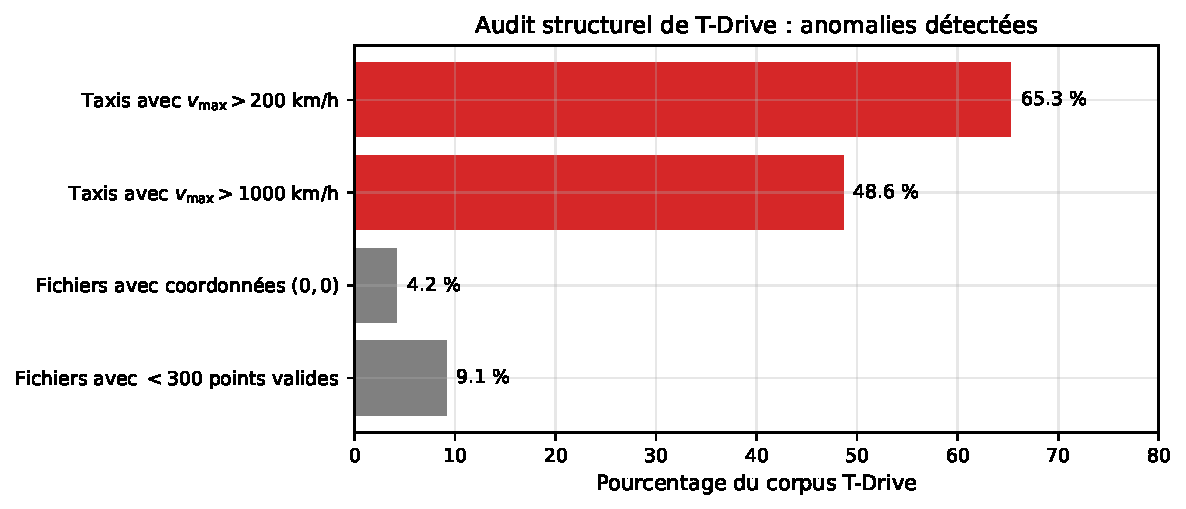
\includegraphics[width=0.85\textwidth]{graphe_6_tdrive.pdf}
\caption{Audit structurel de T-Drive. 65{,}3~\% des 10\,289 taxis présentent des vitesses
maximales supérieures à $200$~km/h et 48{,}6~\% dépassent $1\,000$~km/h, ce qui est
incompatible avec un trafic urbain. Ces artefacts rendent T-Drive inutilisable pour
l'estimation de $H$ sur la série des distances inter-points.}
\label{fig:tdrive}
\end{figure}

Les deux premières lignes sont rédhibitoires (figure~\ref{fig:tdrive}). Une inspection
manuelle de 10 fichiers confirme ces chiffres : le fichier \code{log\_segment\_0.txt} du
taxi 6275 montre des sauts de 1\,495~km (Sichuan) sans déplacement physique, avec des
vitesses instantanées de $5{,}38 \times 10^6$~km/h. Avec $T_{\mathrm{gap}}=900$~s, la taille
médiane des segments T-Drive est de 10 points ; même à 1\,800~s, elle n'atteint que 21
points. T-Drive est donc structurellement incompatible avec l'estimation de $H$ sur la série
des distances $d_i$. Cette conclusion est factuelle : elle repose sur un calcul, pas sur une
affirmation de la littérature.

Nous avons aussi testé T-Drive pour les lois de puissance. Les fichiers ont été convertis au
format interne après filtrage des taxis à pas médian aberrant (pas hors de $[30,700]$~s) :
9\,307 taxis sur 10\,357 sont retenus, soit 17,6 millions de points. Le pipeline standard
(arrêts de 200~m et 20~min, comme pour GeoLife) détecte 165\,591 séjours et 126\,601 paires
de distances. La distribution des durées est dominée par les stationnements nocturnes : le
seuil $x_{\min}$ ajusté par la méthode de Clauset vaut 12{,}7~h, et la queue ne contient que
1{,}8~\% des séjours (2\,018 sur 110\,521). Avec une durée minimale d'arrêt de 300~s, le
phénomène s'aggrave : la queue tombe à 0{,}06~\% des séjours (2\,063 sur 3\,186\,489), et
$x_{\min}$ reste à 12{,}6~h. Pour les distances, $x_{\min}$ vaut 16{,}5~km : la queue mesure
des courses entières de taxi, pas des déplacements entre activités. Dans les deux cas,
l'ajustement est rejeté ($p_{\text{boot}} < 0{,}001$) et l'exposant ajusté ($\alpha = 4{,}9$
pour les séjours, $2{,}8$ pour les distances) ne décrit pas la mobilité humaine.
T-Drive mesure l'exploitation d'une flotte, pas la mobilité résiduelle. Nous l'écartons donc
de toutes les analyses qui suivent.

\subsection{Chiffres de référence}

Sauf mention contraire, tous les résultats de ce mémoire portent sur GeoLife, avec
\code{TIME\_GAP\_THRESHOLD = 900} et \code{MIN\_POINTS = 300}. Le
tableau~\ref{tab:corpus} donne les chiffres de référence.

\begin{table}[ht]
\centering
\caption{Chiffres de référence du corpus analysé.}
\label{tab:corpus}
\small
\begin{tabular}{lr}
\toprule
Indicateur & Valeur \\
\midrule
Utilisateurs avec au moins un segment retenu & 145 \\
Segments retenus & 19\,150 \\
Segments gardés (critère strict) & 7\,853 (41,0~\%) \\
Utilisateurs avec au moins un segment gardé & 136 \\
Utilisateurs sans aucun segment gardé & 9 \\
Concentration des segments gardés (top 5 utilisateurs) & 25,4~\% \\
\bottomrule
\end{tabular}
\end{table}

Deux nombres proches désignent des populations différentes. Les 136 utilisateurs avec au
moins un segment gardé dépendent du filtre de fiabilité sur $H$
(section~\ref{sec:circularite}). Les 137 utilisateurs avec au moins un arrêt détecté, que
nous utilisons pour les lois de puissance, dépendent de la durée minimale d'arrêt de
1\,200~s. Ces deux ensembles diffèrent par leur composition autant que par leur taille.

% =====================================================================
\section{Méthodes}
\label{sec:methodes}
% =====================================================================

\subsection{Prétraitement des trajectoires}
\label{sec:prep}

\subsubsection{Principes}

Quatre principes guident le prétraitement. Nous \emph{marquons avant de décider} : les
points suspects sont signalés dans les fichiers de sortie sans être retirés, et l'effet
d'une coupure est mesuré à part. Nous préférons des \emph{seuils relatifs au contexte du
segment}, calculés localement et bornés par des planchers ou des plafonds absolus. Nous
écrivons \emph{deux versions de chaque estimateur}, l'une de référence et lisible, l'autre
vectorisée, reliées par des tests de parité. Enfin, tout est \emph{traçable} : chaque ligne
de résultats porte une empreinte des constantes de configuration, de sorte que changer une
seule constante change l'empreinte, et les simulations partent d'une graine dérivée.

\subsubsection{Lecture, nettoyage et doublons}

Les six lignes d'en-tête sont ignorées. La date et l'heure sont converties en secondes UNIX
\emph{en UTC}, comme les labels GeoLife. Un point est rejeté si sa latitude n'est pas dans
$[-90,90]$ ou sa longitude hors de $[-180,180]$. L'ordre des opérations est : nettoyage,
tri par horodatage, puis suppression des doublons en gardant le premier. Cette dernière
étape a un défaut : seul l'horodatage est testé, de sorte que si deux positions distinctes
portent le même horodatage, la seconde est perdue (la documentation de la fonction parle,
à tort, de « même position et même horodatage »).

\subsubsection{Segmentation par trous temporels}

Un trou $t_i-t_{i-1} > T_{\mathrm{gap}} = 900$~s ouvre un nouveau segment. Nous
n'interpolons pas et nous ne raccordons jamais deux segments : combler un trou ou raccorder
deux morceaux fabrique un saut artificiel dans la série des distances, auquel la DFA est
très sensible~\cite{chen2002}.

La littérature ne donne pas de seuil unique pour segmenter des trajectoires GPS. Nous avons
donc mesuré, sur le corpus, la proportion de points conservés pour chaque couple
$(T_{\mathrm{gap}}, N_{\min})$ (figure~\ref{fig:heatmap}). La distribution des écarts
temporels $\Delta t$ (figure~\ref{fig:deltas}) montre un pic à 1--10~s, qui correspond à la
résolution native des horodatages, puis une décroissance monotone : \emph{aucun pic naturel}
ne désigne un seuil. Toute valeur doit donc reposer sur une contrainte externe.

\begin{figure}[ht]
\centering
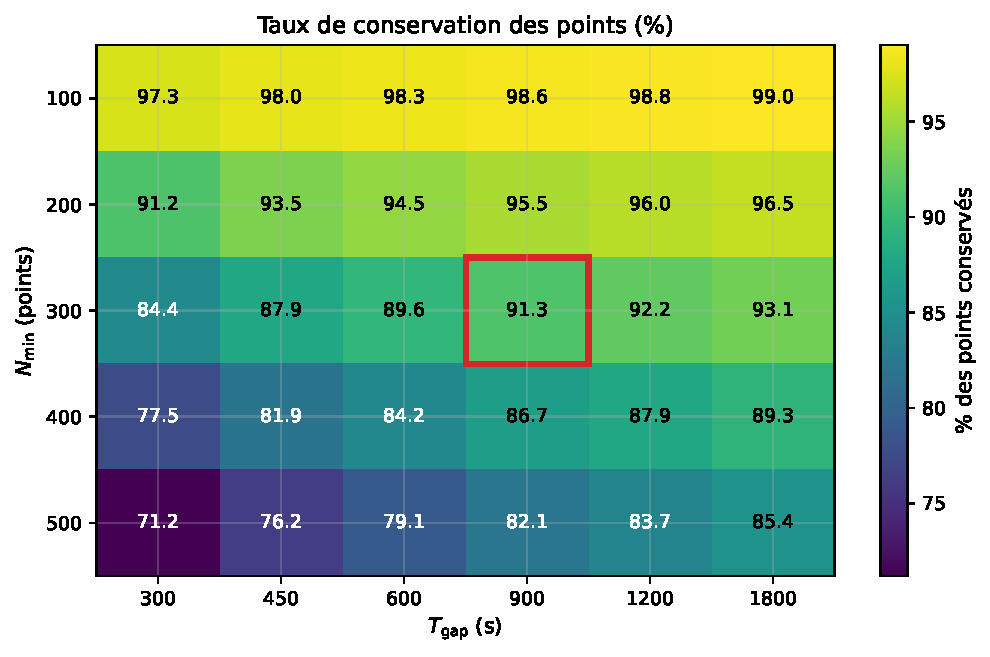
\includegraphics[width=0.8\textwidth]{graphe_5_heatmap.pdf}
\caption{Taux de conservation des points (\%) en fonction du seuil de segmentation
$T_{\mathrm{gap}}$ et du minimum de points $N_{\min}$. Le couple retenu $(900, 300)$
est dans une zone de $91{,}3\,\%$ de conservation, entouré de valeurs proches
($89{,}6$ à $600$~s, $92{,}2$ à $1\,200$~s). Cette continuité indique que la décision
n'est pas sensible à de petites variations.}
\label{fig:heatmap}
\end{figure}

\begin{figure}[ht]
\centering
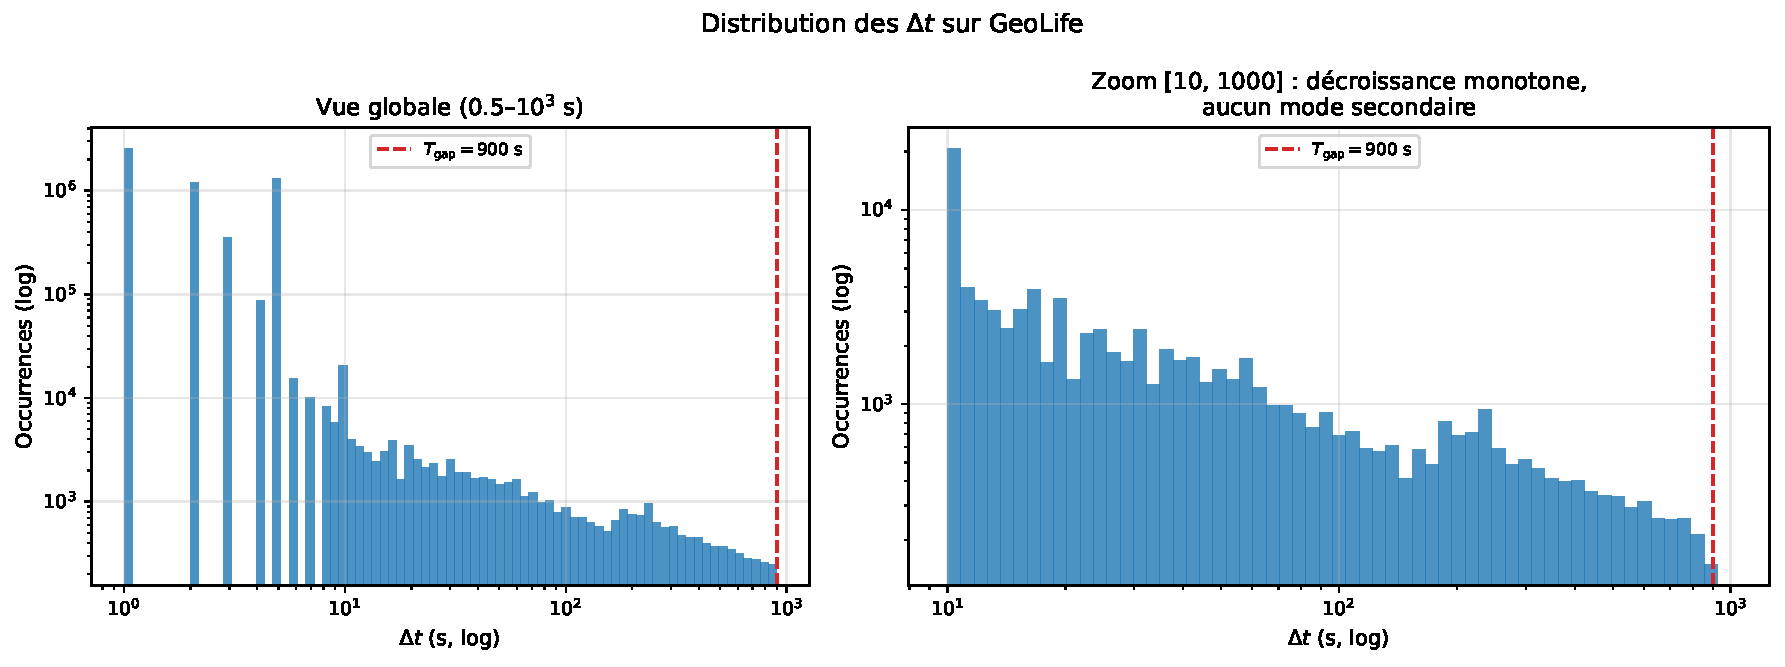
\includegraphics[width=\textwidth]{graphe_8_deltas.pdf}
\caption{Distribution des intervalles $\Delta t$ entre points successifs sur GeoLife
(échelle log-log). Les pics à 1--10~s correspondent à la résolution native des
horodatages. Au-delà de 10~s, la distribution est monotone décroissante, sans mode
secondaire.}
\label{fig:deltas}
\end{figure}

Nous retenons $T_{\mathrm{gap}}=900$~s et $N_{\min}=300$. À ce point, 91,3~\% des points
sont conservés dans des segments qui satisfont les deux critères, et la taille médiane des
segments retenus est de 721 points (figure~\ref{fig:longueurs}). Un segment doit contenir
assez de points pour que la DFA dispose de plusieurs échelles, sans qu'exiger davantage ne
vide le corpus. Le seuil de 900~s ne fragmente pas les trajectoires en segments de quelques
minutes et reste très en deçà des trous d'enregistrement typiques de GeoLife (plusieurs
heures à plusieurs jours). Ce choix est une décision d'ingénierie fondée sur ces chiffres,
pas une recommandation de la littérature ; un couple 600/200 serait tout aussi défendable,
avec plus de segments mais une DFA moins fiable sur chacun. Notons que 900~s n'a pas été
testé sur d'autres corpus.

\subsubsection{Statistiques de segment et stationnarité}

Pour un segment de $N$ points, nous calculons la distance $d_i$ (formule de Haversine),
l'intervalle $\delta_i=t_i-t_{i-1}$ et la vitesse $v_i=d_i/(\delta_i/3600)$ en km/h. Deux
indicateurs en découlent : $R=\sigma_v/\tilde v$ (hétérogénéité des vitesses, où $\tilde v$
est la vitesse médiane) et $\rho=\bar d_2/\bar d_1$, rapport des distances moyennes des deux
moitiés, que nous gardons pour l'affichage seulement.

La stationnarité est jugée par un test de Kolmogorov--Smirnov à deux échantillons entre les
deux moitiés de la série des distances. Ce test a une limite sérieuse. Pour une série
stationnaire à mémoire longue, la variance de la moyenne empirique décroît comme $N^{2H-2}$,
plus lentement que $N^{-1}$, et les deux moitiés peuvent s'écarter davantage que sous
l'indépendance. Le test peut donc rejeter la stationnarité d'une série stationnaire
persistante, c'est-à-dire du cas étudié. Sur le corpus, la $p$-valeur du test est inférieure
à $10^{-20}$ pour la quasi-totalité des segments gardés : l'indicateur discrimine peu.

\subsubsection{Marquage des points suspects}

Le tableau~\ref{tab:seuils} résume les seuils du marquage.

\begin{table}[ht]
\centering
\caption{Principaux seuils du marquage ($\tilde d$ et $\tilde v$ : distance et vitesse
médianes du segment ; $N$ : nombre de points).}
\label{tab:seuils}
\small
\begin{tabular}{p{4.6cm}p{8.4cm}}
\toprule
Composant & Seuil \\
\midrule
Saut de distance & $\min(30\times\tilde d,\;500)$ m \\
Vitesse maximale & $\min\bigl(200,\;\max(5,\;20\times\tilde v)\bigr)$ km/h \\
Variation brutale de vitesse & $\max(20,\;5\times\mathrm{MAD}_v)$ km/h \\
Persistance d'un régime & $\max(5,\;\mathrm{round}(0{,}01\,N))$ points \\
Repli si $\mathrm{MAD}=0$ & $\max(5,\;3\tilde v)$ km/h \\
Stationnarité & test KS à deux échantillons sur les deux moitiés \\
\bottomrule
\end{tabular}
\end{table}

Un point est marqué \code{suspect\_dist} si $d_i$ dépasse le seuil de saut de distance, ce
qui détecte les sauts de position grossiers indépendamment de la vitesse. Pour la vitesse,
nous utilisons le Z-score modifié d'Iglewicz et Hoaglin~\cite{iglewicz1993},
$Z_i = 0{,}6745\,(v_i-\tilde v)/\mathrm{MAD}$ avec $\mathrm{MAD}=\mathrm{med}(|v_i-\tilde v|)$.
Un point est candidat si $Z_i>3{,}5$ ; le calcul est asymétrique, car seules les vitesses
au-dessus de la médiane sont candidates. Un garde-fou absolu classe en \code{artefact} tout
point dont la vitesse dépasse le seuil de vitesse maximale du tableau~\ref{tab:seuils}.

Chaque candidat est ensuite classé selon sa variation locale de vitesse $\Delta v$ et sa
persistance, c'est-à-dire le nombre de points consécutifs au-dessus du seuil
(tableau~\ref{tab:classes}). Le raisonnement est le suivant : un pic brutal et isolé est
probablement une erreur de mesure, tandis qu'une vitesse élevée qui dure est un changement
réel de comportement. Seuls les points \code{artefact} et \code{suspect\_dist} servent de
points de coupure dans la variante par morceaux de l'estimation de $H$ ; les points
\code{regime} n'en sont jamais.

\begin{table}[ht]
\centering
\caption{Classification des points candidats.}
\label{tab:classes}
\small
\begin{tabular}{@{}lll@{}}
\toprule
Variation $\Delta v$ & Persistance & Classe \\
\midrule
brutale ($>5 \times \mathrm{MAD}_v$) & isolée ($<5$ points) & \code{artefact} \\
quelconque & soutenue ($\ge5$ points) & \code{regime} (premier point seul marqué) \\
modérée & isolée & non marqué \\
\bottomrule
\end{tabular}
\end{table}

Ce marquage a une faiblesse que le code rend visible. Le seuil de vitesse est plafonné à
200~km/h mais vaut vingt fois la vitesse médiane : dans un segment surtout piéton dont la
médiane est de 3~km/h, il tombe autour de 60~km/h. Un trajet motorisé soutenu au sein d'un
tel segment risque donc d'être classé en \code{artefact} plutôt qu'en \code{regime}, et de
devenir un point de coupure. Nous n'avons pas mesuré cet effet sur le corpus.

Sur le corpus (145 utilisateurs, 19\,150 segments retenus, 21\,960\,883 points), le marquage
touche les volumes du tableau~\ref{tab:marquage}. Comme le seuil de distance est relatif à
la médiane du segment, ces volumes sont plus élevés qu'avec des seuils absolus.

\begin{table}[ht]
\centering
\caption{Volume de points marqués sur le corpus.}
\label{tab:marquage}
\small
\begin{tabular}{lrr}
\toprule
Marquage & Points marqués & Fraction du corpus \\
\midrule
\code{suspect\_dist}    & 148\,203 & 0,67~\% \\
\code{suspect\_vitesse} & 273\,499 & 1,25~\% \\
\bottomrule
\end{tabular}
\end{table}

\subsubsection{Sélection finale des segments}

Deux filtres retiennent les segments exploitables : au moins $N_{\min}=300$ points, et une
distance parcourue minimale (0,1~km au plus bas ; dans la configuration par défaut, ce
seuil est relatif au pas d'échantillonnage et atteint environ 0,6~km pour un pas de 7~s).
Le seuil de 300 points coupe une minorité de segments : 66~\% des segments retenus ont
moins de 1\,000 points, et la médiane est de 721 (figure~\ref{fig:longueurs}). Elle reste
toutefois bien en deçà des longueurs souvent recommandées pour une estimation stable de
$H$ (voir par exemple~\cite{eke2002}). Nous assumons cette limite.

\begin{figure}[ht]
\centering
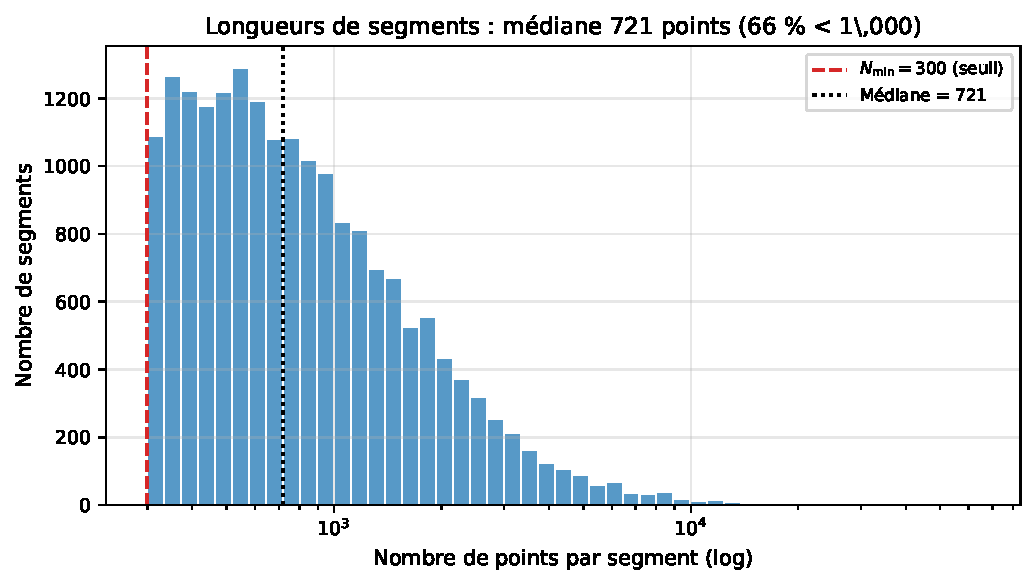
\includegraphics[width=0.75\textwidth]{graphe_7_longueurs.pdf}
\caption{Distribution des longueurs de segments retenus (échelle log). La médiane est
de 721 points, au-dessus du seuil $N_{\min} = 300$. 66~\% des segments ont moins
de $1\,000$ points : le seuil coupe une minorité, mais la plupart des segments restent
courts au regard des longueurs recommandées pour estimer $H$ de façon stable.}
\label{fig:longueurs}
\end{figure}

Ces filtres s'appliquent \emph{avant} la détection d'arrêts. Ils éliminent donc les segments
courts et les segments quasi immobiles où un long séjour a été enregistré : les séjours que
nous analysons sont sélectionnés selon la longueur du segment qui les contient. De plus, le
seuil de 300 points correspond à des durées très différentes selon le mode d'enregistrement
(5~minutes à 1~s, 50~minutes à 10~s). Enfin, il exclut 37 utilisateurs (environ 20~\%), aux
profils variés : segments maximaux trop courts (148, 32, 180, 235 points, etc.) ou points
insuffisants. Ce seuil se justifie par la stabilité de la DFA, mais rien ne le justifie pour
les lois de puissance : un utilisateur dont le plus long segment compte 148 points peut avoir
plusieurs arrêts et distances exploitables. Nous n'avons pas quantifié l'effet de cette
exclusion sur l'exposant $\alpha$ agrégé.

\subsubsection{Mode d'enregistrement}

Une heuristique classe un fichier en mode \emph{temps} si au moins 60~\% des pas ont un
intervalle à $\pm 20$~\% de la médiane, et en mode \emph{distance} si au moins 50~\% des
pas en mouvement ont une distance à $\pm 30$~\% de la médiane. Le mode peut changer à
l'intérieur d'un fichier.

\subsection{Détection d'arrêts et temps de séjour}
\label{sec:arrets}

Nous construisons deux variables : le \emph{temps de séjour}, et la \emph{distance entre deux
arrêts consécutifs}. L'algorithme est une fenêtre ancrée, d'après Li et al.~\cite{li2008}
employé sur des trajectoires GPS dans~\cite{zheng2009}. Pour chaque point $p_i$ pris comme
ancre, on cherche le premier indice $j$ tel que $\mathrm{dist}(p_i,p_j)>R_{\mathrm{arr}}$. Si
$t_j-t_i\ge T_{\min}$, on déclare un arrêt, localisé au centroïde des points de la fenêtre.

Deux écoles coexistent dans la littérature : 100~m et 5~min d'un côté, 200~m et 20 à 30~min
de l'autre (Zheng et al.). GeoLife étant le corpus de référence de cette seconde école, nous
adoptons $R_{\mathrm{arr}}=200$~m et $T_{\min}=1200$~s (20~min). Nous mesurons la sensibilité
à ce choix sur quatre couples : $(100, 300)$, $(100, 600)$, $(200, 1200)$ et $(200, 1800)$
(section~\ref{sec:lp-sensibilite}).

\paragraph{Observation finie et censure.}\label{sec:censure} Suivant Kivelä et
Porter~\cite{kivela2015}, nous n'écartons pas les durées biaisées : nous les étiquetons
(colonne \code{censuree}). Un arrêt qui commence au premier point d'un morceau est
\emph{censuré à gauche}. Un arrêt jamais suivi d'une sortie du rayon n'est pas détecté,
sauf si l'on active l'option correspondante. Les \emph{pauses entre segments} sont
récupérées à part. Pour l'ajustement des lois, nous ne gardons par défaut que les arrêts
internes non censurés.

\paragraph{Deux variantes de distance.} Nous écartons les distances inférieures à 100~m.
Nous distinguons ensuite deux variables. La variable \code{distance} ne contient que les
paires d'arrêts situés dans le \emph{même segment}, sans trou entre eux : c'est la variante
« propre ». La variable \code{distance\_a\_cheval} contient aussi les paires séparées par un
trou d'enregistrement : c'est la variante « large ». La restriction au même segment élimine
environ 87~\% des paires du corpus (1\,283 paires conservées sur 10\,216), ce qui rend la
variante propre peu exploitable statistiquement. Nous discutons ce compromis à la
section~\ref{sec:lp-resultats}.

\paragraph{Limites.} Trois défauts de cette détection sont connus. La détection s'exécute sur
les segments retenus : les segments courts et quasi immobiles en sont absents. Le bruit GPS
peut faire sortir un point du rayon et couper artificiellement un long séjour en deux ; le
second morceau est alors tronqué sans être étiqueté censuré, ce qui fausse la queue de la
distribution, précisément ce que nous cherchons à estimer. Enfin, la durée inclut le pas de
sortie du rayon, ce qui la surestime, surtout près de $T_{\min}$.

\subsection{Estimation de $H$ par segment et filtre de fiabilité}
\label{sec:est}

\subsubsection{Série et paramètres}

La série analysée est $d_1,\dots,d_{N-1}$, les distances entre points successifs (une option
permet d'analyser les vitesses $v_i$ à titre de contrôle). Nous avons suivi le cahier des
charges, qui impose cette série. Son défaut est de mélanger vitesse et intervalle de temps
($d_i=v_i\delta_i$) : elle mesure l'intensité du déplacement, pas sa direction.

La DFA utilise 20 échelles de $s_{\min}=4$ à $\lfloor N/4\rfloor$. Nous calculons aussi les
pentes des moitiés basse et haute de la courbe, leur écart, et des pentes locales sur des
fenêtres de 5 échelles. Le R/S utilise des blocs de 10 à $\lfloor N/2\rfloor$. Le Whittle
local retient $m=\min(\lfloor N^{0,65}\rfloor, \lfloor N/4\rfloor)$ fréquences sur la grille
de la section~\ref{sec:whittle}. Pour chaque segment, nous écrivons $\hat H$ par méthode et
des colonnes de fiabilité : dépassement de 1 par la DFA, indicateur de borne du Whittle,
résultats du test de dépassement, mode d'enregistrement. Nous calculons enfin la
\emph{divergence} entre méthodes, c'est-à-dire l'écart entre la plus grande et la plus
petite estimation disponibles. Dans le filtre et dans cette divergence, la pente R/S utilisée
est la pente brute.

\subsubsection{Deux critères de sélection}

Deux critères coexistent dans le code, et nous les distinguons dans ce texte. Le drapeau
\code{suspect} vaut 1 si la divergence dépasse $0{,}15$, ou si $\hat H_{\mathrm{DFA}}>1$, ou
si $\hat H_{\mathrm{RS}}>1$, ou si $\hat H_{\mathrm{Whittle}}>0{,}999$. Le critère
\emph{gardé}, plus strict, est celui du filtre de fiabilité. Un segment est gardé si et
seulement si les quatre conditions suivantes sont réunies :
\begin{enumerate}
  \item les trois méthodes ont produit une valeur ;
  \item $0 < \hat H < 1$ pour chacune des trois méthodes ;
  \item le minimum de $R(H)$ du Whittle n'est pas sur une borne de la grille
  (\code{whittle\_a\_la\_borne} faux) ;
  \item la divergence est au plus de $0{,}15$.
\end{enumerate}
Dans la pratique, les deux critères coïncident sur la quasi-totalité des segments. Sur
19\,150 segments retenus et 145 utilisateurs, 7\,853 segments sont gardés (41,0~\%), et
97,1~\% d'entre eux sont aussi \emph{forts}, c'est-à-dire que les trois méthodes donnent
$H>0{,}5$.

\subsubsection{Circularité du filtre}
\label{sec:circularite}

C'est la limite la plus importante du mémoire. Le filtre porte sur le résultat lui-même : la
condition sur la divergence utilise les valeurs de $\hat H$ des trois méthodes, et les
conditions de bornes utilisent également $\hat H$. L'écart moyen
$|\hat H_{\mathrm{DFA}} - \hat H_{\mathrm{RS}}|$ passe de $0{,}079$ sur l'ensemble des
utilisateurs à $0{,}023$ sur les utilisateurs gardés (moyenne par utilisateur). Le même
calcul par segment donne $0{,}152 \to 0{,}058$. Dans les deux cas, cette réduction est
acquise \emph{par construction} : ce n'est pas une confirmation indépendante de l'accord
des méthodes. La figure~\ref{fig:circularite} le rend visible : les segments gardés se
concentrent dans la bande $|\Delta H| \leq 0{,}15$ non parce que les méthodes concordent
d'elles-mêmes, mais parce que cette bande est le critère de sélection. Le $\hat H$ des
segments gardés doit donc se lire comme un $\hat H$ \emph{conditionnel au filtre}, pas comme
un $\hat H$ de population.

\begin{figure}[ht]
\centering
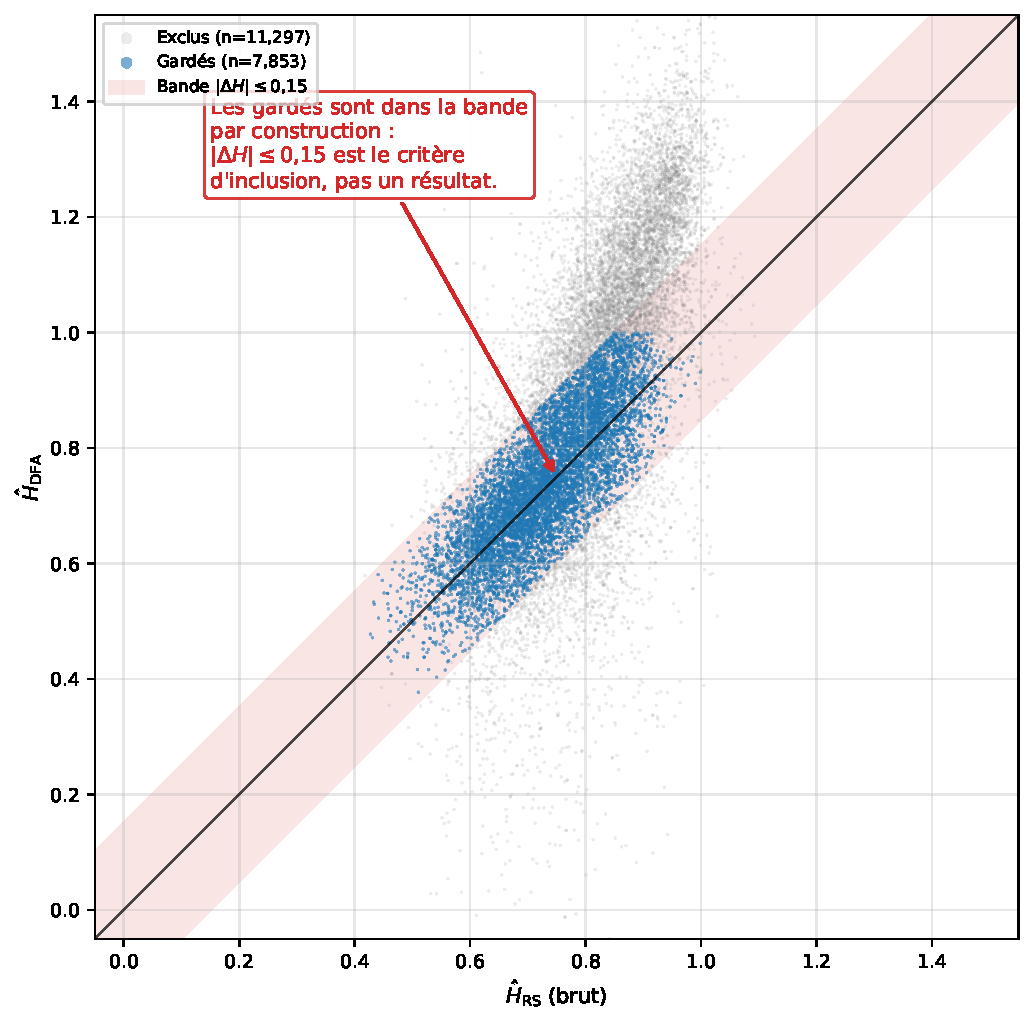
\includegraphics[width=0.75\textwidth]{graphe_3_circularite.pdf}
\caption{$\hat H_{\mathrm{DFA}}$ contre $\hat H_{\mathrm{RS}}$ pour tous les segments,
coloriés selon le critère de garde. Les segments gardés sont concentrés dans la bande
$|\Delta H| \leq 0{,}15$ \emph{par construction} : cette bande est le critère
d'inclusion, non un résultat de la convergence indépendante des méthodes.}
\label{fig:circularite}
\end{figure}

\subsubsection{Variante par morceaux}

Nous calculons aussi $\hat H_{\mathrm{morceaux}}$ : la DFA après coupure du segment aux
points \code{artefact} et \code{suspect\_dist}, sans raccord, puis combinée par une moyenne
pondérée par la longueur des morceaux. Dans le script d'estimation, un morceau doit compter
au moins 20 points ; la constante de configuration de 50 points n'est utilisée que par
l'expérience de sensibilité.

\subsection{Test de dépassement d'un modèle à mémoire courte}
\label{sec:nul}

Ce test compare la pente DFA observée à celles de séries à mémoire courte de même longueur
et de même distribution. La procédure comporte quatre étapes :
\begin{enumerate}
  \item transformer la série en loi normale à partir de ses rangs ;
  \item ajuster un AR($p$) par Yule--Walker, avec $p\le p_{\max}$ choisi par l'AIC ;
  \item simuler 99 séries AR($p$) de même longueur ;
  \item leur redonner exactement la distribution de valeurs de la série observée, par
  échange de rangs.
\end{enumerate}
La $p$-valeur est la proportion de surrogats dont la pente est au moins égale à la pente
observée, avec $+1$ au numérateur et au dénominateur ; elle est unilatérale. Nous rapportons
le test pour $p_{\max}=1$ et $p_{\max}=5$.

Il faut bien lire ce que ce test dit. Il indique qu'une dépendance n'est \emph{pas expliquée
par un AR($p$)}. Il ne prouve pas la mémoire longue, car une alternance de régimes produit
le même rejet~\cite{diebold2001}. Nous ne l'utilisons donc jamais comme argument suffisant.

\subsection{Lois de puissance : protocole}
\label{sec:lp-methode}

\subsubsection{Ajustement de Clauset}

Nous suivons la méthode de Clauset et al.~\cite{clauset2009}. Pour un $x_{\min}$ donné, on
calcule le maximum de vraisemblance de $\alpha$ ; on retient le $x_{\min}$ qui minimise la
distance de Kolmogorov--Smirnov parmi au plus 200 seuils candidats, la queue devant compter
au moins 50 points. L'adéquation est testée par un bootstrap semi-paramétrique de
1\,000 simulations, dans lequel $x_{\min}$ est réestimé à chaque simulation. La loi est
\emph{rejetée} si la $p$-valeur est $\le 0{,}1$.

\subsubsection{Lois alternatives et test d'adéquation de la tronquée}

Nous ajustons quatre alternatives sur la même queue : exponentielle, log-normale, Weibull et
loi de puissance à coupure exponentielle. Chacune est comparée à la loi de puissance pure par
un rapport de log-vraisemblance (section~\ref{sec:notions}), et nous calculons des poids
d'Akaike corrigés~\cite{burnham2002}.

Le meilleur poids d'Akaike dit quelle loi est la meilleure \emph{du catalogue}, pas qu'elle
s'ajuste bien. Pour répondre à cette seconde question, nous appliquons à la loi tronquée un
test d'adéquation par bootstrap paramétrique (200 simulations). Ce test diffère de celui de
Clauset : $x_{\min}$ y est fixé à sa valeur observée au lieu d'être réestimé, et seuls
$\alpha$ et $\lambda$ sont réajustés. Il coûte environ trois fois moins cher, mais il est
moins sensible à un mauvais choix de seuil et il est beaucoup moins exigeant. Un $p>0{,}1$
sur ce test ne prouve donc \emph{pas} que la tronquée est adéquate. Un $p\le0{,}1$ est en
revanche un rejet net. Ses résultats ne sont pas directement comparables à ceux du test de
Clauset, qui porte sur la loi pure.

\subsubsection{Verdicts et populations}

Chaque distribution reçoit un verdict : \code{rejetee}, \code{alternative\_meilleure},
\code{plausible}, \code{insuffisant} ou \code{indetermine}. « Plausible » signifie seulement
que la loi n'est pas rejetée : d'autres lois peuvent l'être tout autant. L'ajustement est
fait sur l'ensemble des utilisateurs agrégés, puis séparément pour chaque utilisateur ayant
au moins 100 observations. Pour chaque ajustement, nous calculons l'exposant de survie
$a=\alpha-1$ et nous indiquons si $\alpha$ appartient au domaine $2<\alpha<3$ de la
relation~\eqref{eq:onoff}.

\subsubsection{Limites de la méthode}

Trois limites s'appliquent. D'abord, le bootstrap suppose des observations indépendantes,
alors que les durées d'une même personne sont probablement corrélées. L'agrégation
d'utilisateurs hétérogènes mélange en outre des lois différentes : Yan et al.~\cite{yan2013}
montrent qu'une loi de puissance à coupure exponentielle peut émerger de l'agrégation
d'individus hétérogènes dont la plupart ne suivent pas eux-mêmes de loi d'échelle. Une
tronquée sur données agrégées ne prouve donc pas que chaque individu est scale-free.
Ensuite, l'exclusion des durées censurées retire les plus longues et biaise l'exposant vers
le haut ; la correction naturelle, une vraisemblance avec censure, n'est pas implémentée.
Enfin, une queue minimale de 50 points rend le choix de $x_{\min}$ instable pour les petits
utilisateurs, et le seuil de $0{,}1$ est appliqué à de nombreux utilisateurs sans correction
pour tests multiples.

% =====================================================================
\section{Validation sur séries simulées}
\label{sec:valid}
% =====================================================================

\subsection{Exactitude des estimateurs}
\label{sec:exactitude}

Les séries de $H$ connu sont générées exactement par plongement circulant de la covariance,
selon Davies et Harte~\cite{davies1987} ; un fBm s'obtient par somme cumulée du fGn. Un
catalogue de modèles à mémoire courte (AR(1), moyenne à changements de régime) et un
processus ON/OFF à durées de Pareto complète le dispositif. Pour chaque couple $(H_0,N)$,
nous générons 200 réalisations d'un fGn, nous estimons $H$ par quatre variantes (DFA, R/S
brut, R/S corrigé, Whittle) et nous résumons le biais et la RMSE. Le
tableau~\ref{tab:exactitude} donne les cellules utiles à l'interprétation du corpus ; la
figure~\ref{fig:validation} montre l'ensemble.

\begin{table}[ht]
\centering
\caption{Biais et RMSE des estimateurs sur fGn de $H_0$ connu (200 réalisations par cellule, graine 20261018).}
\label{tab:exactitude}
\small
\begin{tabular}{rrrrrrrrr}
\toprule
$H_0$ & $N$ & \multicolumn{2}{c}{DFA} & \multicolumn{2}{c}{R/S corrigé} & \multicolumn{2}{c}{Whittle} \\
 & & biais & RMSE & biais & RMSE & biais & RMSE \\
\midrule
0{,}5 & 300 & $+0{,}032$ & $0{,}065$ & $+0{,}004$ & $0{,}056$ & $+0{,}002$ & $0{,}091$ \\
0{,}7 & 300 & $+0{,}011$ & $0{,}061$ & $-0{,}065$ & $0{,}093$ & $-0{,}000$ & $0{,}095$ \\
0{,}9 & 300 & $+0{,}011$ & $0{,}067$ & $-0{,}149$ & $0{,}161$ & $-0{,}002$ & $0{,}081$ \\
0{,}7 & 1000 & $+0{,}007$ & $0{,}039$ & $-0{,}048$ & $0{,}063$ & $-0{,}001$ & $0{,}059$ \\
0{,}9 & 1000 & $+0{,}002$ & $0{,}045$ & $-0{,}121$ & $0{,}127$ & $+0{,}001$ & $0{,}052$ \\
\bottomrule
\end{tabular}
\end{table}

\begin{figure}[ht]
\centering
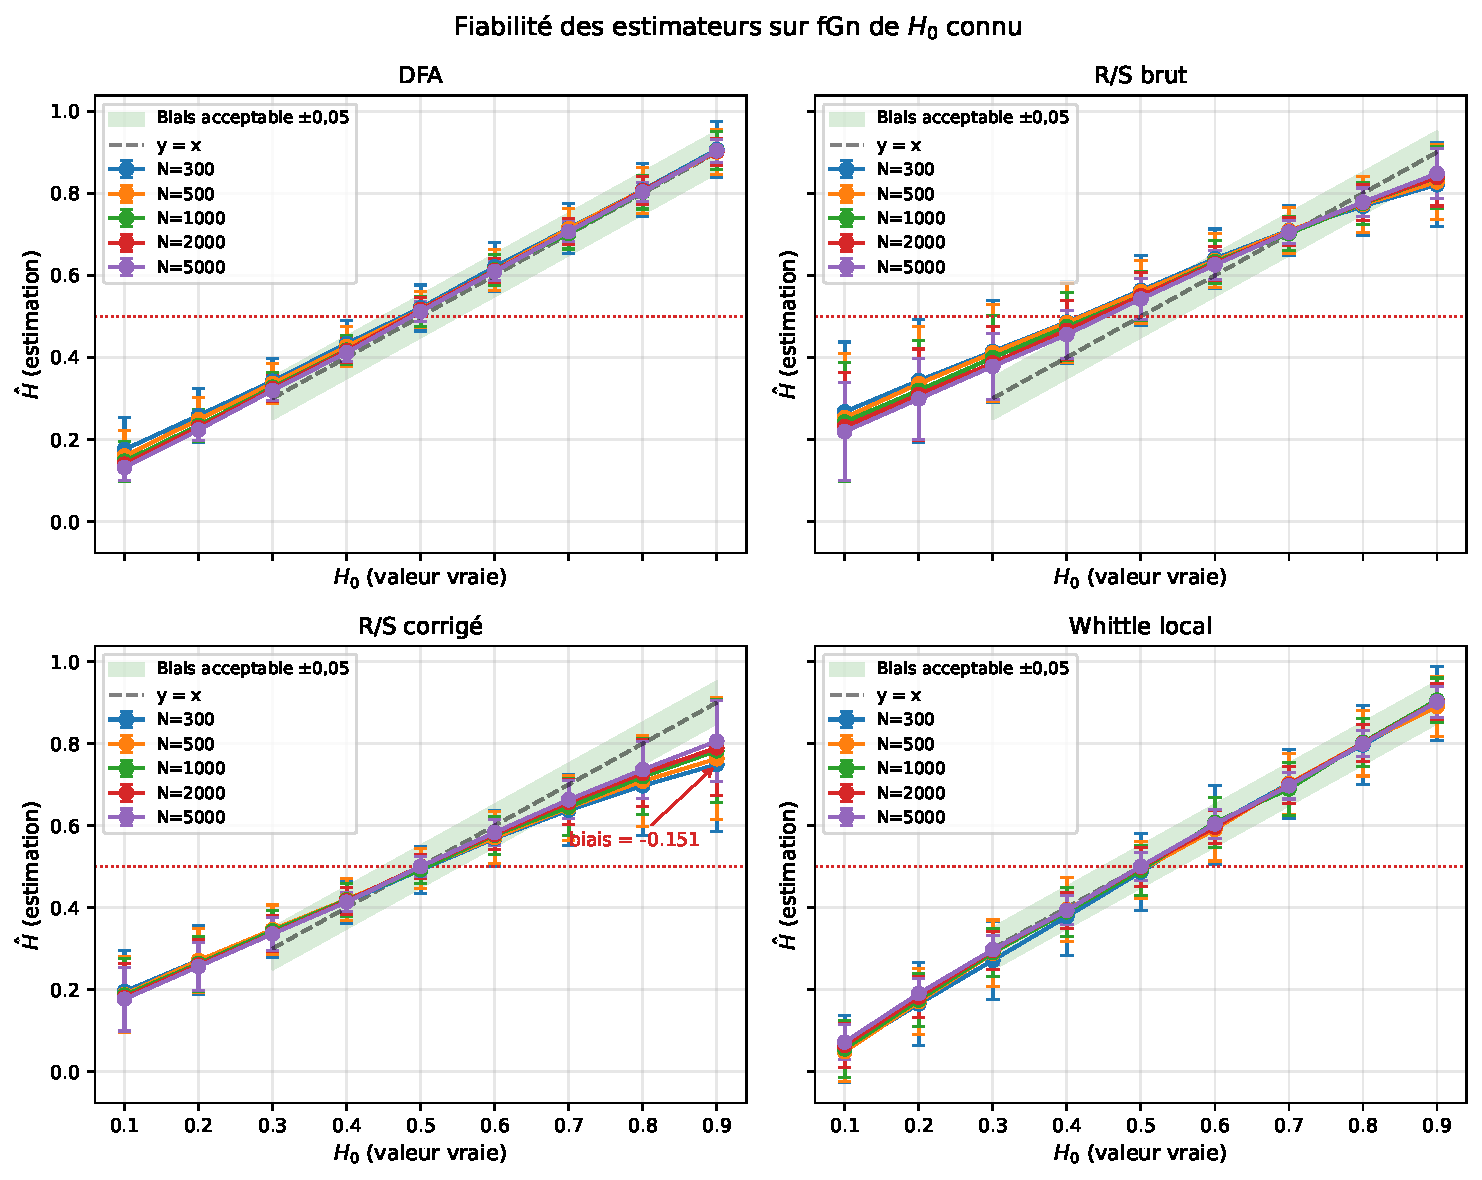
\includegraphics[width=\textwidth]{graphe_1_validation.pdf}
\caption{Biais et RMSE des quatre variantes d'estimation sur des fGn de $H_0$ connu
(200 répliques par cellule). DFA et Whittle suivent la diagonale ; le R/S corrigé
(Anis--Lloyd) sous-estime les séries persistantes au-delà de $H_0 = 0{,}7$
(biais $-0{,}149$ à $N=300$, $H_0=0{,}9$).}
\label{fig:validation}
\end{figure}

La lecture est nette. Le biais de la DFA et celui du Whittle sont proches de zéro sur tout
le domaine testé. Leur dispersion reste modérée : la RMSE de la DFA ne dépasse pas $0{,}067$
à $N=300$ ni $0{,}045$ à $N=1000$ ; celle du Whittle atteint $0{,}095$ à $N=300$ et
$0{,}059$ à $N=1000$. Le R/S corrigé est fiable pour $H\le0{,}5$ mais devient inutilisable
comme référence à partir de $H=0{,}7$ : la correction d'Anis--Lloyd, conçue pour un bruit
sans mémoire, sur-corrige les séries persistantes. Ce biais mesuré, qui se retrouve sur 2\,400
séries synthétiques (4 valeurs de $H_0$, 3 longueurs, 200 répliques), justifie de ne pas
prendre le R/S comme référence indépendante pour valider un $H$ élevé.

\subsection{Hypothèses testées et verdicts}
\label{sec:hypotheses}

Nous avons formulé sept hypothèses, chacune avec un seuil fixé avant le test. Le
tableau~\ref{tab:hypotheses} rapporte tous les verdicts, y compris ceux qui ne sont pas des
confirmations.

\begin{table}[ht]
\centering
\caption{Hypothèses testées, seuils pré-fixés et verdicts.}
\label{tab:hypotheses}
\small
\begin{tabular}{p{0.9cm}p{4.4cm}p{2.6cm}p{5.2cm}}
\toprule
\textbf{Hyp.} & \textbf{Énoncé} & \textbf{Seuil pré-fixé} & \textbf{Verdict} \\
\midrule
H1 & Estimateurs fiables sur fGn & $|\text{biais}| < 0{,}05$ & DFA/Whittle confirmés, R/S infirmé à $H \ge 0{,}7$ \\
H2 & Régime $\to$ rejet du nul AR($p$) & taux de rejet $\ge 0{,}5$ & Confirmée pour $p_{\max}=1$ ($N=1000$ : 100~\%), non pour $p_{\max}=5$ (19~\%) ; partielle à $N=300$ (76~\% ; 6~\%) \\
H3 & Corrélation $\rho_1$--$H$ & $|\rho_S| > 0{,}5$ & Confirmée ($\rho_S = 0{,}859$) \\
H4 & AR(1) reproduit les taux du corpus & $\Delta T < 10$~pts & Infirmée (corpus 20,3~\% ; $\phi=0{,}5$ et $\phi=0{,}8$ : 2 à 6~\%) \\
H5 & Mobile/non-mobile à $\rho_1$ fixé & $|\Delta| < 0{,}10$ & Confirmée mais fragile ($\Delta = +0{,}057$) \\
H6 & Test nul calibré à $\rho_1 = 0$ & $\in [0{,}03, 0{,}07]$ & Confirmée (5{,}25~\%) \\
H7 & Corpus invalide pour $H$ & fraction $< 0{,}10$ & Infirmée (82{,}9~\% valides) \\
\bottomrule
\end{tabular}
\end{table}

\paragraph{H1.} Sur fGn à $H_0=0{,}9$ et $N=300$, le R/S corrigé présente un biais de
$-0{,}149$ et une RMSE de $0{,}161$ : la correction d'Anis--Lloyd sur-corrige à haute
persistance.

\paragraph{H2.} Le modèle \code{regimes} (une moyenne constante par morceaux, de paramètres
figés) déclenche le rejet du nul à $N=1000$ dans 100~\% des cas avec $p_{\max}=1$, mais dans
19~\% seulement avec $p_{\max}=5$ : un ordre AR plus élevé absorbe une partie de
l'autocorrélation artificielle créée par les paliers. À $N=300$, la puissance chute (76~\%
à $p_{\max}=1$, 6~\% à $p_{\max}=5$). La conclusion porte sur ce modèle générique.

\paragraph{H4.} Le taux de rejet du modèle nul sur le corpus est de 20,3~\%. Un AR(1) avec
$\phi=0{,}5$ ou $\phi=0{,}8$ n'en produit que 2 à 6~\% : le corpus ne s'explique donc pas
par les deux AR(1) testés. L'exclusion de toute la famille AR(1) n'est pas établie. En
revanche, ce taux est compatible avec le modèle \code{regimes} (19~\% à $p_{\max}=5$) et avec
un fGn de $H=0{,}6$ (16~\% à $p_{\max}=5$). Le rejet du nul est donc cohérent avec
« régimes » ou « mémoire longue modérée », pas avec « i.i.d. ».

\paragraph{H6.} Sur un modèle i.i.d. ($\rho_1 = 0$), le taux de faux positifs est de
5,25~\%, cohérent avec le seuil nominal de 5~\%. Sur un AR(1) à $\rho_1 = 0{,}5$, il tombe
à 2,5~\% : le test AR($p$) absorbe une partie de la dépendance à court terme et devient plus
conservateur. Cela ne remet pas H6 en cause (qui porte sur $\rho_1 = 0$) mais précise le
comportement du test.

\paragraph{H7.} La fraction de segments valides, définie par $s_{\max}/s_{\min} \ge 4$, est
de 82,9~\%, très au-dessus du seuil de 10~\%. Un critère plus strict, exigeant une décade
complète d'échelles, inverserait la conclusion. L'infirmation porte donc sur la
formulation du critère, pas sur le corpus.

\subsection{Test du mécanisme ON/OFF}
\label{sec:onoff-test}

L'hypothèse de travail est que la dépendance apparente pourrait provenir d'une alternance
mouvement/arrêt à queue de Pareto (section~\ref{sec:onoff}). Un script vérifie d'abord, sur
données simulées, que la DFA et le Whittle retrouvent $H=(3-a)/2$, puis compare sur données
réelles le $H$ mesuré à la prédiction issue de l'exposant des séjours. Dans l'état actuel du
code, cette expérience a un défaut : la fonction de simulation tire un lot entier de durées
avec un seul exposant avant d'alterner les états, ce qui revient à utiliser le même exposant
pour les phases ON et OFF. La partie sur données réelles, qui demande deux exposants
distincts, est donc invalide. Nous ne présentons pas ses résultats ; elle doit être corrigée
puis régénérée.

\subsection{Sensibilité au prétraitement}

Une expérience recalcule $\hat H_{\mathrm{DFA}}$ sur les mêmes segments sous plusieurs
variantes : coupure aux artefacts sans raccord, coupure aux trous de plus de 60~s, coupure
aux intervalles supérieurs à trois fois le pas médian, série des vitesses, échelle minimale
de DFA plus grande, stratification par mode d'enregistrement. Un \emph{placebo} retire le
même nombre de points que la coupure aux artefacts, à des positions aléatoires, pour
vérifier que l'effet observé ne vient pas du seul fait de retirer des points. Cette
expérience est écrite mais nous n'en présentons pas les résultats ici.

% =====================================================================
\section{Résultats}
\label{sec:resultats}
% =====================================================================

\subsection{Exposant de Hurst sur GeoLife}
\label{sec:resultats-H}

Tous les chiffres de cette section sont obtenus avec \code{TIME\_GAP\_THRESHOLD = 900} et
\code{MIN\_POINTS = 300}, sur les 145 utilisateurs ayant au moins un segment retenu.

\subsubsection{Tous les segments, ou seulement les gardés}

\begin{table}[ht]
\centering
\caption{Moyennes de $\hat H$ par méthode, tous segments et segments gardés.}
\label{tab:moyennes-H}
\small
\begin{tabular}{lrrr}
\toprule
Population & $\hat H_{\mathrm{DFA}}$ & $\hat H_{\mathrm{RS}}$ & $\hat H_{\mathrm{Whittle}}$ \\
\midrule
Tous segments (145 utilisateurs) & 0{,}834 & 0{,}776 & 0{,}802 \\
Segments gardés (136 utilisateurs) & \textbf{0{,}726} & \textbf{0{,}723} & \textbf{0{,}728} \\
Segments gardés, pondéré par $n_{\text{gardés}}$ & 0{,}741 & 0{,}731 & 0{,}740 \\
\bottomrule
\end{tabular}
\end{table}

Le filtre agit surtout sur la DFA (figure~\ref{fig:distribution}). Il fait baisser sa
moyenne de $0{,}11$ et sa médiane de $0{,}12$ : c'est la méthode la plus sensible à la
non-stationnarité. Le R/S baisse de $0{,}05$ et le Whittle de $0{,}07$. L'écart entre la
moyenne arithmétique (par utilisateur) et la moyenne pondérée (par segment) reflète la
concentration des segments gardés : les cinq plus gros utilisateurs en portent 25,4~\%, et
leurs $H$ sont supérieurs à la moyenne.

\begin{figure}[ht]
\centering
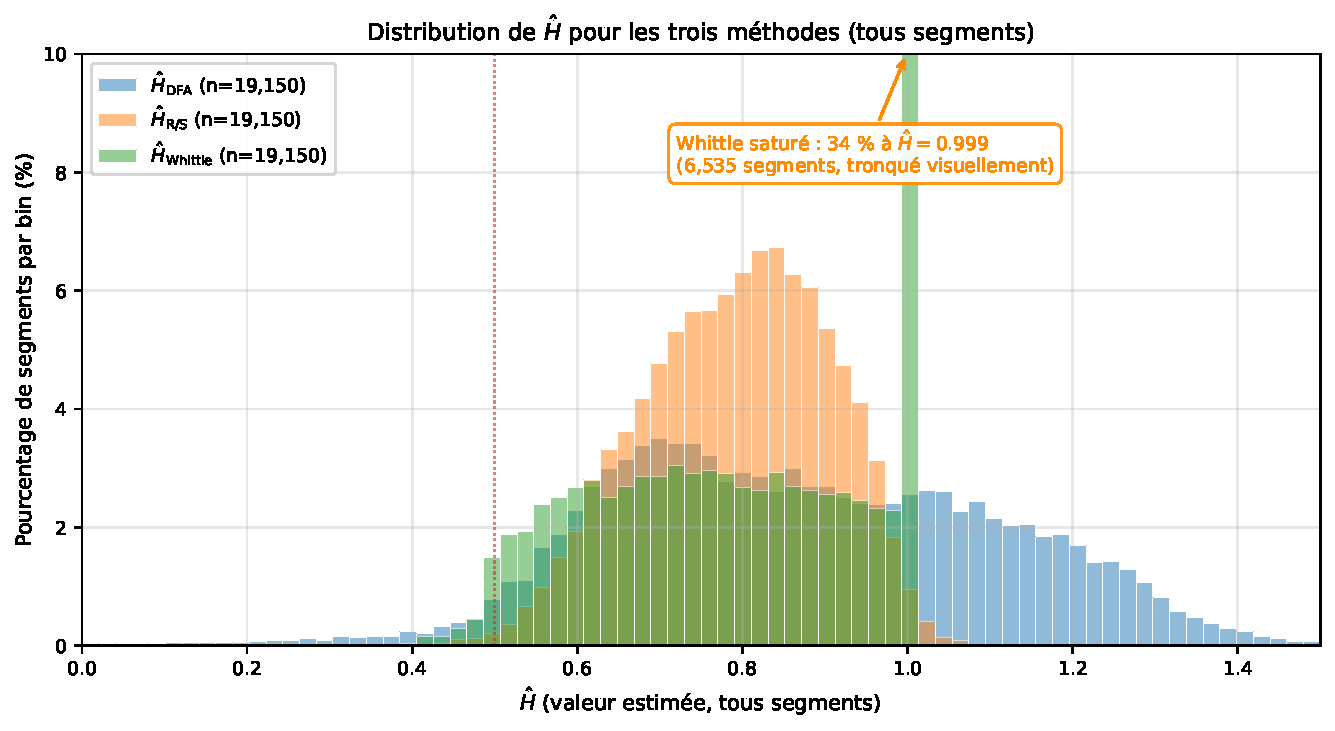
\includegraphics[width=\textwidth]{graphe_2_distribution.pdf}
\caption{Distribution de $\hat H$ sur les 19\,150 segments retenus (gris) et les
7\,853 segments gardés (bleu), pour les trois méthodes. Le filtre élimine la queue
super-diffusive ($\hat H > 1$) et la saturation du Whittle ($\hat H = 1$, $n = 5\,365$),
et déplace la médiane de $0{,}857$ à $0{,}736$ (DFA). Ce déplacement n'est pas une
amélioration de la précision : c'est un changement de population.}
\label{fig:distribution}
\end{figure}

\subsubsection{Concentration et dispersion}

\begin{table}[ht]
\centering
\caption{Dispersion de $\hat H_{\mathrm{DFA}}$ sur les segments gardés, par strate d'effectif.}
\label{tab:dispersion}
\small
\begin{tabular}{lrr}
\toprule
Strate & Nombre d'utilisateurs & $\hat H_{\mathrm{DFA}}$ (moyenne $\pm$ écart-type) \\
\midrule
$n_{\text{gardés}} \ge 50$ & 43 & $0{,}738 \pm 0{,}038$ \\
$n_{\text{gardés}} < 10$ & 45 & $0{,}712 \pm 0{,}096$ \\
\bottomrule
\end{tabular}
\end{table}

La dispersion observée est compatible avec un bruit d'échantillonnage dominant : les
utilisateurs à faible effectif ont une variance plus grande. Elle n'exclut pas une
hétérogénéité réelle résiduelle. La figure~\ref{fig:user_ic} le montre : les intervalles
de confiance des utilisateurs à faible effectif se recouvrent largement, ce qui rend leur
ordre non significatif. La ligne indique la moyenne pondérée des médianes par utilisateur
(0,743), à ne pas confondre avec la moyenne pondérée de tous les segments (0,741).

\begin{figure}[ht]
\centering
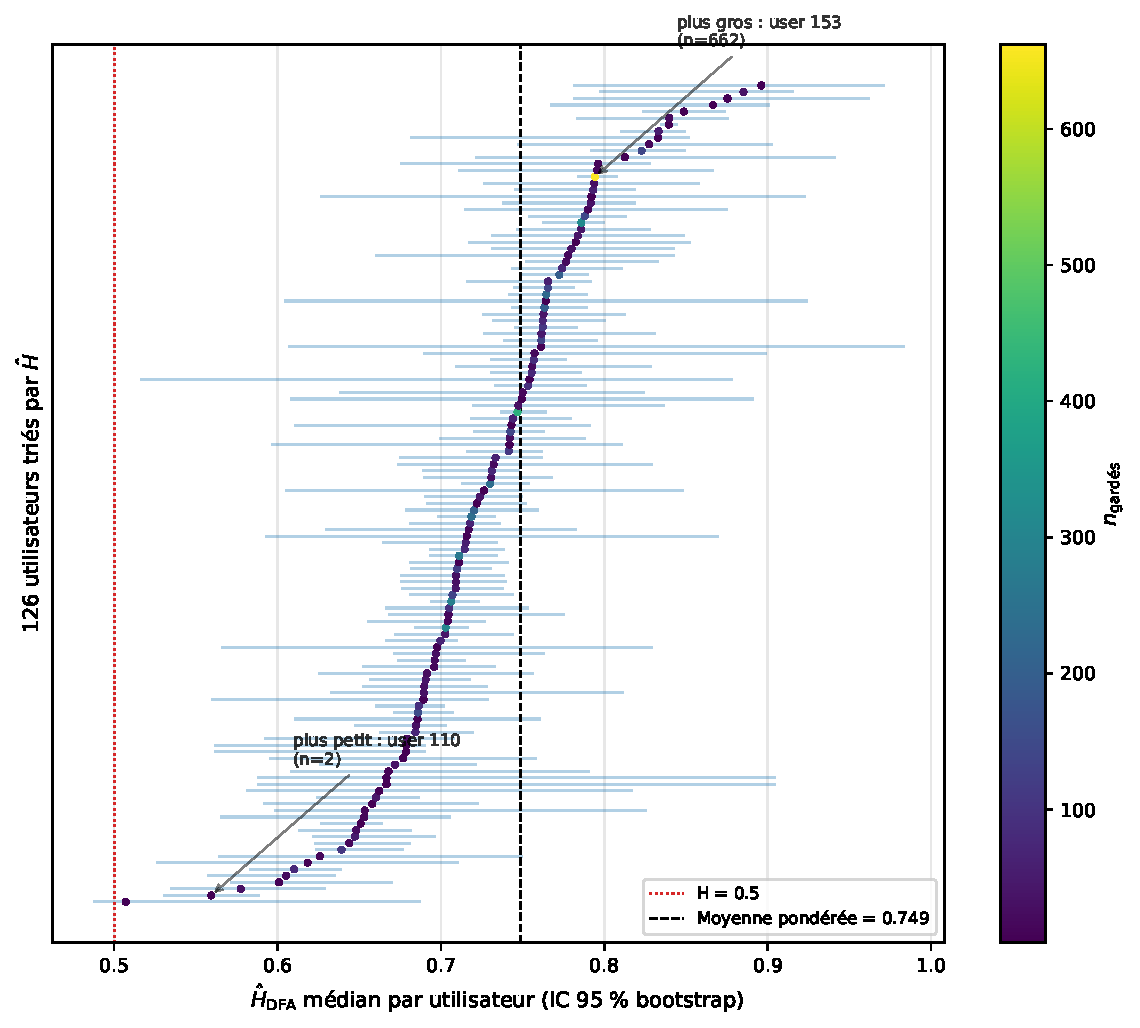
\includegraphics[width=0.8\textwidth]{graphe_4_user_ic.pdf}
\caption{$\hat H_{\mathrm{DFA}}$ médian par utilisateur (126 utilisateurs avec au moins
2 segments gardés), trié par valeur croissante, avec intervalle de confiance à 95\,\%
obtenu par bootstrap sur les segments ($B = 1\,000$). La couleur encode le nombre de
segments gardés. La largeur des intervalles décroît avec $n_{\text{gardés}}$ : la
dispersion inter-utilisateurs est en grande partie du bruit d'échantillonnage.}
\label{fig:user_ic}
\end{figure}

\subsubsection{Neuf utilisateurs sans segment gardé, et doublons}

Neuf utilisateurs (049, 056, 079, 114, 120, 137, 151, 157, 166) n'ont aucun segment gardé.
Six d'entre eux ont $\hat H_{\mathrm{DFA}} > 1$ sur la totalité de leurs segments : leur
trajectoire est super-diffusive sur l'ensemble du fichier. Trois cas sont marginaux : 151 et
157 (1 segment chacun, $\hat H_{\mathrm{DFA}} < 1$) et 120 (5 segments,
$\hat H_{\mathrm{DFA}} = 0{,}90$). Ces utilisateurs ne reçoivent aucune valeur de $H$ dans le
cadre du filtre strict ; ils peuvent représenter un régime balistique légitime plutôt que du
bruit.

Trois paires d'utilisateurs ont des lignes strictement identiques dans la synthèse
($055/075$, $058/059$, $069/129$), et une paire partage le même $\hat H$ des gardés avec des
totaux différents ($046/121$). Nous n'avons pas identifié l'origine de ces doublons
(fichiers source dupliqués, ou problème en amont). Ils représentent 39 segments gardés
(0,50~\%), un volume négligeable, mais à documenter avant toute agrégation
inter-utilisateurs.

\subsubsection{Synthèse}

\begin{table}[ht]
\centering
\caption{Synthèse des estimations sur GeoLife (\code{TIME\_GAP}=900).}
\label{tab:synthese}
\small
\begin{tabular}{lr}
\toprule
Indicateur & Valeur \\
\midrule
Segments retenus & 19\,150 \\
Segments gardés & 7\,853 (41,0~\%) \\
Utilisateurs avec au moins un gardé & 136 \\
$\hat H_{\mathrm{DFA}}$ (moyenne par utilisateur) & 0{,}726 \\
$\hat H_{\mathrm{DFA}}$ (pondéré par $n_{\text{gardés}}$) & 0{,}741 \\
Convergence DFA~$/$~Whittle sur les gardés & $\pm 0{,}02$ \\
Biais du R/S corrigé à $H \ge 0{,}7$ (mesuré sur fGn) & $-0{,}15$ \\
\bottomrule
\end{tabular}
\end{table}

Ce qu'il faut retenir est simple : la valeur $\hat H_{\mathrm{DFA}} \approx 0{,}726$ n'est
\emph{pas} une estimation de la mémoire longue du déplacement. Elle mesure ce que la DFA
produit sur la série $d_i$ filtrée. Le test décisif, à $\rho_1$ contrôlé, a montré que la DFA
\emph{peut} distinguer un fGn d'un AR(1) de même $\rho_1$, mais avec un écart d'environ
$0{,}07$, du même ordre que la RMSE d'estimation. La séparation est donc statistique (sur
19\,150 segments), pas pratique (segment par segment).

\subsection{Lois de puissance sur GeoLife}
\label{sec:lp-resultats}

\subsubsection{Configuration et résultats agrégés}

Nous analysons \textbf{137 utilisateurs} de GeoLife : ceux pour lesquels au moins un arrêt a
été détecté. Sur les 145 utilisateurs ayant un segment retenu, huit n'ont aucune pause de
1\,200~s ou plus dans un rayon de 200~m (021, 049, 102, 116, 118, 166, 170, 173). Ce chiffre
de 137 est distinct des 136 utilisateurs « avec au moins un segment gardé » du critère sur
$H$. Le jeu de seuils est celui par défaut ($R_{\mathrm{arr}} = 200$~m,
$T_{\min} = 1200$~s). Les $p$-valeurs de Clauset sont obtenues avec 1\,000 simulations, et
les alternatives sont activées. Le tableau~\ref{tab:lp-agrege} donne les résultats agrégés.

\begin{table}[ht]
\centering
\caption{Résultats agrégés des lois de puissance sur 137 utilisateurs (jeu 200~m~/~20~min,
$B=1000$ pour le test de Clauset). Entre parenthèses : poids d'Akaike du meilleur modèle.}
\label{tab:lp-agrege}
\small\setlength{\tabcolsep}{4pt}
\begin{tabular}{lrrrll}
\toprule
Variable & $n$ & $\alpha$ & $p_{\text{boot}}$ & Verdict & Meilleur AICc \\
\midrule
\code{sejour} & 5\,354 & $3{,}186 \pm 0{,}031$ & $0{,}159$ & alternative meilleure & tronquée (0{,}967) \\
\code{distance} (même seg.) & 1\,283 & $2{,}026 \pm 0{,}084$ & $0{,}055$ & rejetée & loi pure (0{,}528) \\
\code{sejour\_avec\_censurees} & 13\,378 & $2{,}365 \pm 0{,}029$ & $<0{,}001$ & rejetée & loi pure (0{,}577) \\
\code{distance\_a\_cheval} & 10\,216 & $1{,}779 \pm 0{,}012$ & $<0{,}001$ & rejetée & tronquée (0{,}511) \\
\bottomrule
\end{tabular}
\end{table}

\begin{figure}[ht]
\centering
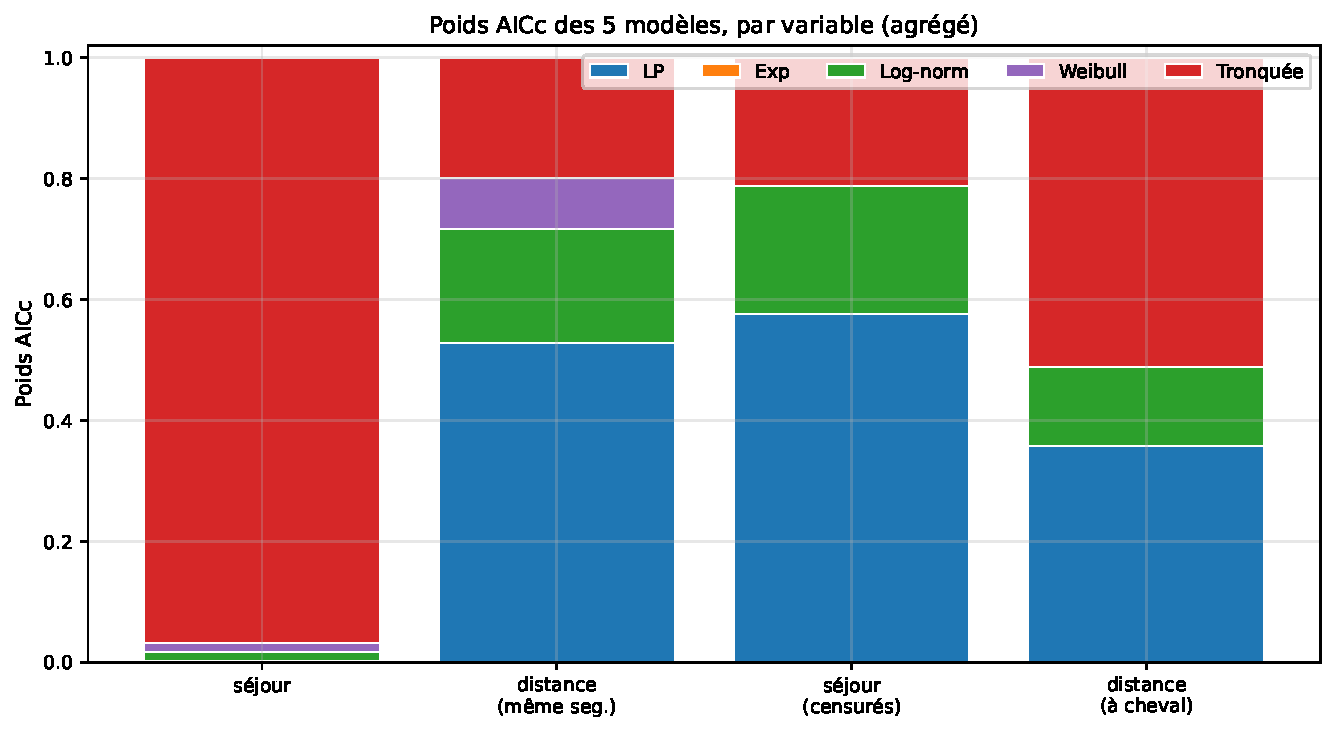
\includegraphics[width=\linewidth]{graphe_10_aicc.pdf}
\caption{Poids d'Akaike corrigés (AICc) des cinq modèles, par variable (population
agrégée, $x \geq x_{\min}$). Chaque barre somme à 1. La loi de puissance pure (bleu) l'emporte
pour \code{distance} (même segment) et \code{sejour\_avec\_censurees}, avec des poids modestes
(0,53 et 0,58). La loi tronquée (rouge) l'emporte pour \code{sejour} et
\code{distance\_a\_cheval}.}
\label{fig:lp-aicc}
\end{figure}

Le classement par AICc dépend de la variable (figure~\ref{fig:lp-aicc}). La loi de puissance
pure est la mieux classée pour deux variables, mais avec un poids proche de 0,5 : aucun
modèle ne s'impose nettement. Pour les deux autres, c'est la loi tronquée qui gagne, avec un
poids de 0,967 pour les séjours et de 0,511 pour les distances à cheval. Le rapport de
vraisemblance en sa faveur est très net pour les séjours ($p_{\mathrm{RV}} = 0{,}0002$) mais
seulement marginal pour les distances à cheval ($p_{\mathrm{RV}} = 0{,}099$, qui ne passe
pas le seuil de 5~\%).

\subsubsection{La loi gagnante est-elle adéquate ?}

Le poids d'Akaike classe les modèles entre eux ; il ne dit pas si le gagnant s'ajuste bien.
Nous regardons donc deux tests d'adéquation. Pour la loi de puissance pure, le test de
Clauset (figure~\ref{fig:lp-pvalues}) ne rejette pas \code{sejour} (sa $p$-valeur est de
$0{,}159$) mais rejette les trois autres variables. Pour la loi tronquée, le
test par bootstrap décrit à la section~\ref{sec:lp-methode} donne le
tableau~\ref{tab:lp-adequation}.

\begin{figure}[ht]
\centering
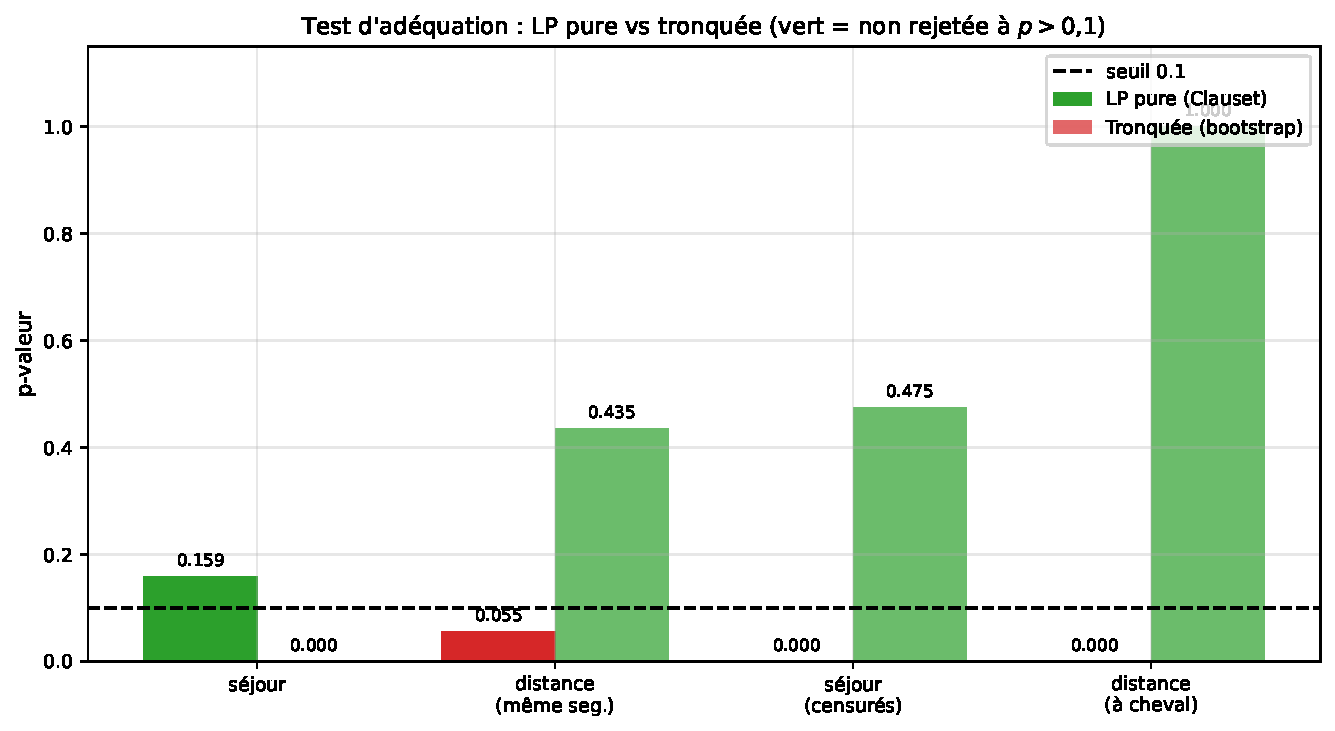
\includegraphics[width=0.85\linewidth]{graphe_11_pvalues.pdf}
\caption{Test d'adéquation de la loi de puissance pure (bootstrap de Clauset,
$x_{\min}$ réestimé, $B = 1000$). Vert : non rejetée à $p > 0{,}1$. Seul
\code{sejour} n'est pas rejeté ($p = 0{,}159$) ; les trois autres variables sont
rejetées. Le test d'adéquation de la loi tronquée (tableau~\ref{tab:lp-adequation})
suit une procédure différente et n'est pas directement comparable.}
\label{fig:lp-pvalues}
\end{figure}

\begin{table}[ht]
\centering
\caption{$p$-valeurs d'adéquation de la loi tronquée (bootstrap, $B=200$, $x_{\min}$ fixé).}
\label{tab:lp-adequation}
\small
\begin{tabular}{lrll}
\toprule
Variable & $p_{\text{tronq}}$ & Verdict & Lecture \\
\midrule
\code{sejour} & $<0{,}005$ & rejetée & rejet net \\
\code{distance} (même seg.) & $0{,}435$ & non rejetée & test peu exigeant, sans conclusion \\
\code{sejour\_avec\_censurees} & $0{,}475$ & non rejetée & $\lambda \approx 0$ : équivalente à la loi pure \\
\code{distance\_a\_cheval} & $1{,}000$ & non rejetée & artefact ($\lambda \to 0$) \\
\bottomrule
\end{tabular}
\end{table}

Un seul cas est informatif : \code{sejour}. La loi tronquée y est rejetée à $p<0{,}005$ alors
que le test, peu exigeant, devrait plutôt la laisser passer. Pour
\code{distance\_a\_cheval}, le $p=1{,}000$ est un artefact : le $\lambda$ ajusté vaut
$6{,}58 \times 10^{-9}$~m$^{-1}$ (coupure à $1{,}5 \times 10^5$~km), numériquement nul sur
le domaine observé. La tronquée est alors équivalente à la loi pure, que le test de Clauset
rejette ; le $p=1{,}000$ reflète seulement le peu d'exigence du test. Pour \code{distance}
(même segment) et \code{sejour\_avec\_censurees}, une non-réjection ne prouve pas
l'adéquation : aucune conclusion ferme n'est possible. Ces deux tests n'étant pas
comparables, on ne peut pas non plus lire les valeurs du tableau~\ref{tab:lp-adequation} à
côté de celles de la figure~\ref{fig:lp-pvalues} comme une comparaison de deux modèles.

\subsubsection{Interprétation par variable}

\paragraph{Durées de séjour (\code{sejour}).} Sur 5\,354 séjours non censurés, dont 5\,110
au-dessus de $x_{\min}$, l'exposant de densité est $\hat\alpha = 3{,}186$. Le test de
Clauset ne rejette pas la loi pure ($p=0{,}159$), mais la loi tronquée obtient un poids
d'Akaike de 0{,}967. Son paramètre de coupure vaut $\lambda = 5{,}92 \times 10^{-5}$~s$^{-1}$,
soit une échelle $1/\lambda \approx 4{,}7$~heures. Cette échelle tombe près de la limite
supérieure des durées observées : le maximum est de l'ordre de $2 \times 10^4$~s, environ
5,5~h, et la figure~\ref{fig:lp-ccdf-sejour} ne montre que quelques points au-delà de
$1/\lambda$. Son interprétation est donc ambiguë. Elle est compatible avec une coupure réelle
(au-delà de quelques heures, les durées ne suivent plus une queue de Pareto), mais aussi avec
la fenêtre d'observation finie, qui tronque les séjours les plus longs~\cite{kivela2015}, et
avec un effet de mélange d'utilisateurs hétérogènes~\cite{yan2013}. Les données seules ne
permettent pas de trancher.

\begin{figure}[ht]
\centering
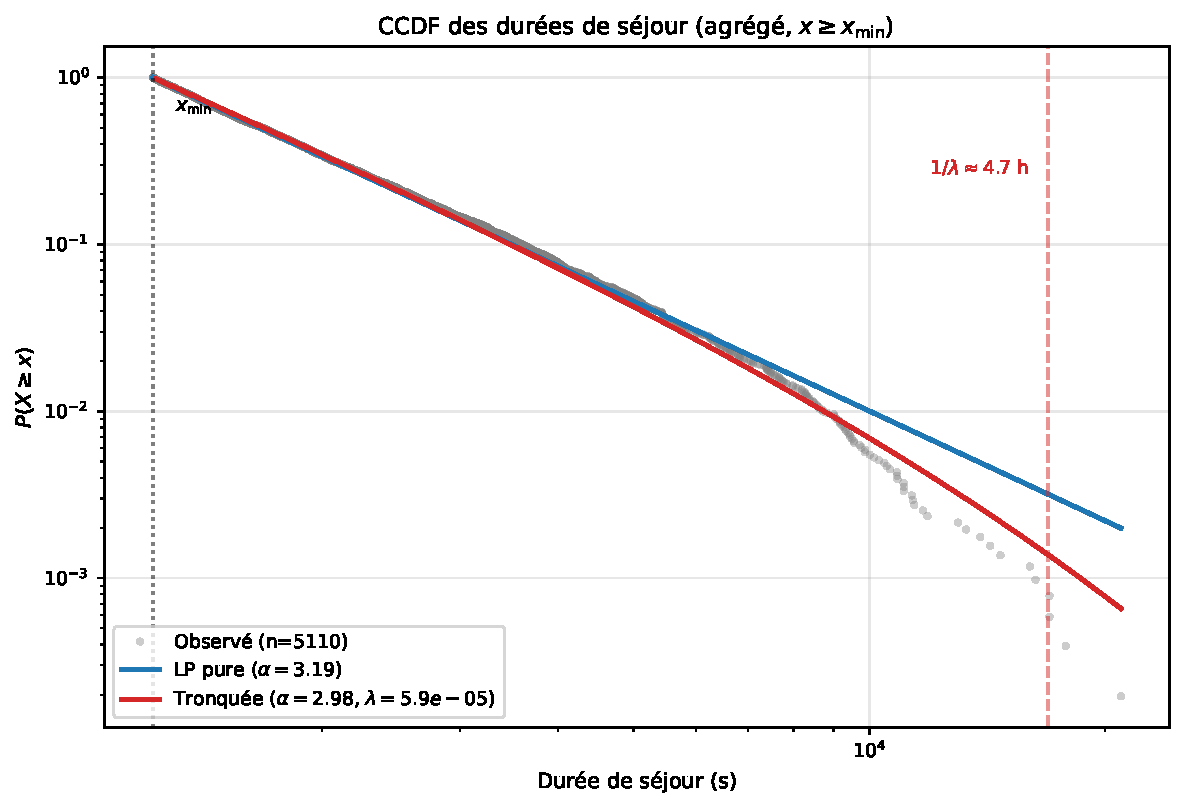
\includegraphics[width=0.85\linewidth]{graphe_9_ccdf_sejour.pdf}
\caption{Fonction de survie empirique des durées de séjour non censurées
($n = 5\,110$ au-dessus de $x_{\min}$), avec les ajustements de la loi de puissance
pure ($\alpha = 3{,}19$) et de la loi tronquée ($\alpha = 2{,}98$,
$\lambda = 5{,}9 \times 10^{-5}$~s$^{-1}$). La ligne verticale rouge marque
$1/\lambda \approx 4{,}7$~h, tout près de la durée maximale observée. Les trois courbes
coïncident jusqu'à environ $7 \times 10^3$~s. Au-delà de $10^4$~s, les données passent sous
les deux modèles, la tronquée comprise, qui descend moins vite que les observations.}
\label{fig:lp-ccdf-sejour}
\end{figure}

La figure~\ref{fig:lp-ccdf-sejour} aide à comprendre le double résultat. La tronquée gagne en
AICc parce qu'elle suit mieux que la loi pure la courbure des données autour de $10^4$~s. Elle
échoue au test d'adéquation parce que les observations plongent ensuite plus vite qu'elle.
Nous en retenons que ni la loi pure (non rejetée par Clauset mais nettement battue en AICc)
ni la loi tronquée (préférée en AICc mais rejetée par bootstrap) ne décrit correctement les
durées de séjour. Les trois autres lois (exponentielle, log-normale, Weibull) ne sont
comparées que par AICc, sans test d'adéquation : on ne peut pas affirmer qu'elles échouent,
seulement qu'elles ne dominent pas le classement.

Notre $\hat\alpha = 3{,}19$ est bien au-dessus de l'exposant d'environ 1,8 que Song et
al.~\cite{song2010} rapportent pour les temps d'attente, avec une coupure vers 17~h. La
comparaison est toutefois délicate : notre exposant est celui d'une loi pure ajustée sur une
queue sélectionnée, alors que le leur est celui d'une loi tronquée (nous trouvons
$\alpha = 2{,}98$ pour la nôtre), sur d'autres données. L'écart peut aussi venir d'un effet de
bord (le filtre des séjours non censurés coupe la queue), du filtre de longueur de segment
appliqué en amont, ou de la définition des arrêts.

\paragraph{Distance dans un même segment (\code{distance}).} Sur 1\,283 paires,
$\hat\alpha = 2{,}026$ et $p_{\text{boot}} = 0{,}055$ : verdict \emph{rejetée}, mais la loi
pure reste la mieux classée en AICc (poids 0{,}528) et aucune alternative ne la bat
nettement. Le cas est ambigu. Avec $B=1000$ (contre $B=500$ dans une version antérieure), le
rejet est confirmé et même renforcé : $p$ passe de $0{,}070$ à $0{,}055$. Sur la
figure~\ref{fig:lp-ccdf-autres}, les points de queue restent au-dessus des courbes : la
queue est plus lourde que celle des deux modèles.

\paragraph{Séjours incluant les censurés (\code{sejour\_avec\_censurees}).} Sur 13\,378
séjours, $\hat\alpha = 2{,}365$ et $p_{\text{boot}} < 0{,}001$ : rejetée. Le $x_{\min}$
ajusté vaut 29\,918~s, environ 8,3~heures : la loi de puissance ne s'ajuste que sur les pauses
de plus de 8~h. Ce n'est pas surprenant, puisque cette variable inclut les \emph{pauses
entre segments}, dont la durée est celle du trou d'enregistrement (appareil éteint). La
distribution est probablement \emph{bimodale} : de vrais séjours, courts, d'un côté, des
absences, longues, de l'autre. L'ajustement place $x_{\min}$ dans la zone des absences,
d'où un $\hat\alpha$ formellement correct mais non interprétable physiquement. Sur la
figure~\ref{fig:lp-ccdf-autres}, la queue suit à peu près une droite sur deux décades, mais
la taille de l'échantillon permet de rejeter l'ajustement. Nous traitons cette variable
comme une variable de sensibilité, pas comme un résultat principal.

\paragraph{Distance à cheval (\code{distance\_a\_cheval}).} Sur 10\,216 paires,
$\hat\alpha = 1{,}779$ et $p_{\text{boot}} < 0{,}001$ : rejetée. La loi tronquée obtient le
meilleur poids (0{,}511), avec un avantage marginal ($p_{\mathrm{RV}} = 0{,}099$). Ce
$\hat\alpha$ est voisin de l'exposant $\beta=1{,}75\pm0{,}15$ rapporté par González et
al.~\cite{gonzalez2008} pour les déplacements, bien que leur loi soit paramétrée
différemment. Le paramètre $\lambda = 6{,}58 \times 10^{-9}$~m$^{-1}$ correspond à une
échelle de $1{,}5 \times 10^5$~km, très au-delà des distances observées ($\le 50$~km) : la
tronquée gagne par flexibilité statistique sur des queues extrêmes peuplées par les sauts à
travers un trou, pas par une coupure physique. La figure~\ref{fig:lp-ccdf-autres} montre un
plateau entre $10^5$ et $2 \times 10^6$~m où les données sont environ trois fois au-dessus
des courbes, suivi d'une coupure brutale vers $10^7$~m (échelle terrestre). Aucune loi du
catalogue ne convient donc à cette variable.

\begin{figure}[ht]
\centering
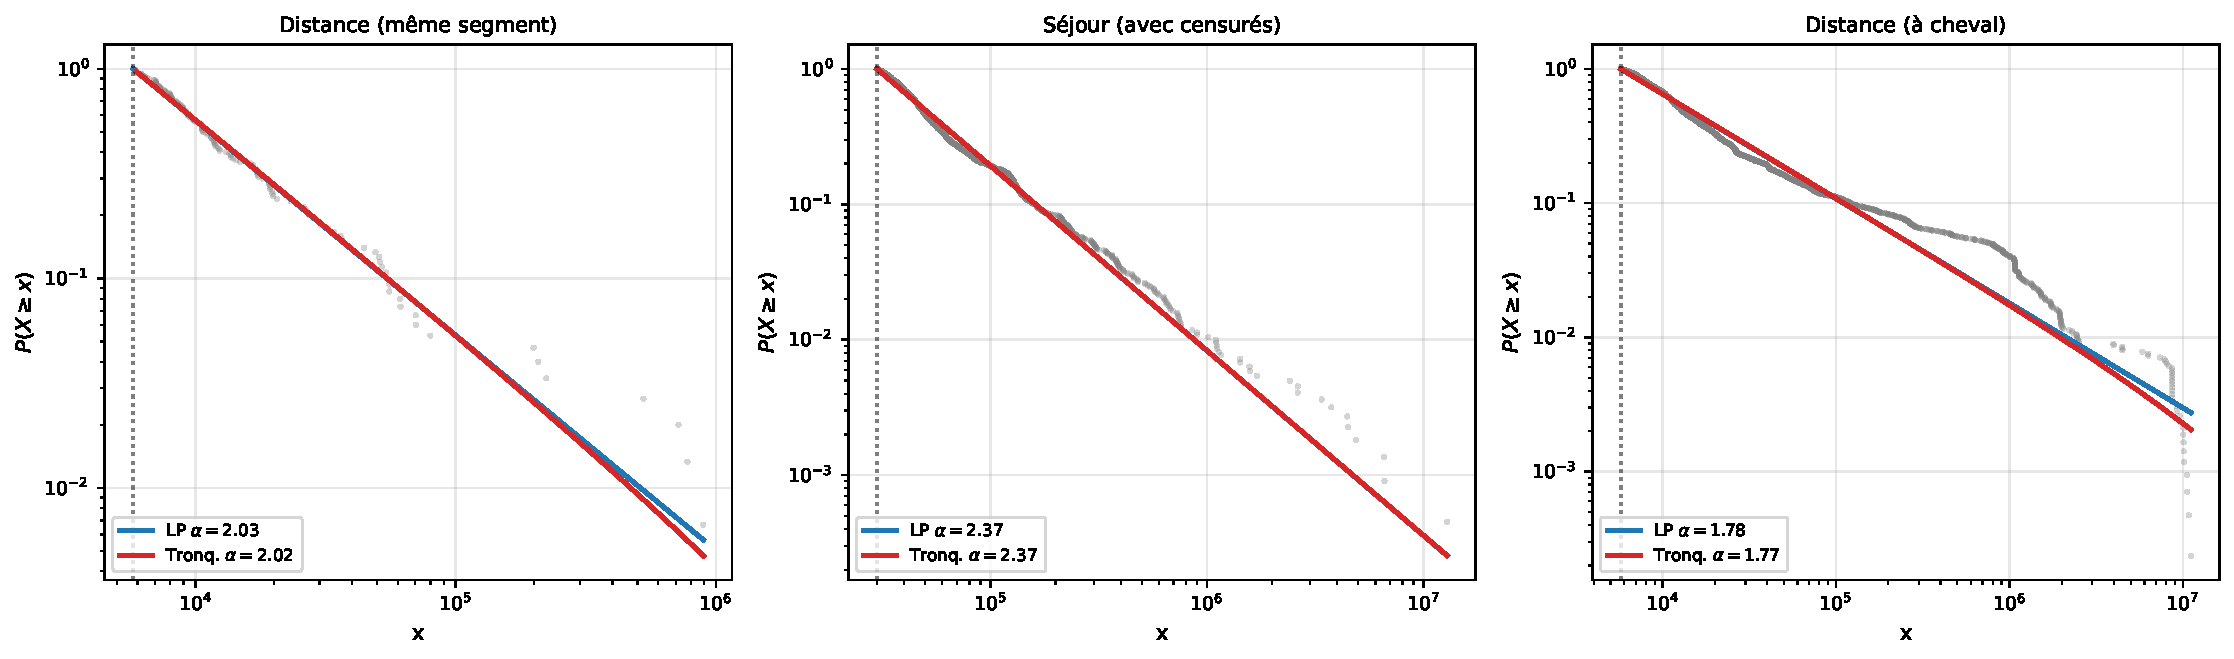
\includegraphics[width=\linewidth]{graphe_13_ccdf_autres.pdf}
\caption{Fonctions de survie empiriques des trois autres variables, avec les
ajustements de la loi de puissance pure (bleu) et de la loi tronquée (rouge).
\emph{Gauche} : distance à l'intérieur d'un même segment (m) : les points de queue
sont au-dessus des courbes (queue plus lourde que les modèles), l'ajustement est
raisonnable jusqu'à $10^5$~m. \emph{Centre} : séjour avec censurés (s) : la queue
est approximativement une droite sur deux décades, mais la taille de
l'échantillon ($n = 13\,378$) permet de rejeter l'ajustement. \emph{Droite} :
distance à cheval (m) : plateau entre $10^5$ et $2 \times 10^6$~m où les données
sont environ trois fois au-dessus des courbes, puis coupure vers $10^7$~m.}
\label{fig:lp-ccdf-autres}
\end{figure}

\paragraph{Distance dans un même segment ou à cheval.} Le choix de la variable est un
arbitrage entre pureté et volume. \code{distance} compte 1\,283 paires sans aucune traversée
de trou, mais elle écarte environ 87~\% des paires, car deux arrêts consécutifs se trouvent
presque toujours dans des segments différents. \code{distance\_a\_cheval} en compte 10\,216,
mais certaines traversent un trou d'enregistrement : des arrêts intermédiaires ont pu passer
inaperçus, ce qui gonfle les distances et abaisse mécaniquement $\hat\alpha$. Nous rapportons
les deux et les lisons comme des bornes : 2,03 pour la première, 1,78 pour la seconde. La
vérité est probablement entre les deux. Retirer les paires qui traversent un trou de plus de
15~min reste à faire.

\subsubsection{Sensibilité aux seuils d'arrêt}
\label{sec:lp-sensibilite}

Comme la segmentation, le jeu de seuils d'arrêt est un arbitrage, pas une prescription de la
littérature. Nous l'avons fait varier sur les quatre couples
$(100, 300)$, $(100, 600)$, $(200, 1200)$ et $(200, 1800)$
(tableau~\ref{tab:lp-sensibilite}, figure~\ref{fig:lp-sensibilite}).

\begin{table}[ht]
\centering
\caption{Sensibilité de $\alpha$ aux quatre jeux de seuils d'arrêt (population
agrégée, $B = 50$ ; les $\sigma_\alpha$ sont de l'ordre de 0{,}02--0{,}05).}
\label{tab:lp-sensibilite}
\small
\begin{tabular}{lrrrr}
\toprule
Jeu & $n_{\text{séjour}}$ & $\alpha_{\text{séjour}}$ & $n_{\text{distance}}$ & $\alpha_{\text{distance}}$ \\
\midrule
100~m~/~5~min  & 32\,110 & 3{,}12 & 13\,806 & 1{,}89 \\
100~m~/~10~min & 14\,185 & 3{,}18 & 4\,064  & 1{,}82 \\
200~m~/~20~min & 5\,354  & 3{,}19 & 1\,283  & 2{,}03 \\
200~m~/~30~min & 2\,789  & 3{,}42 & 428    & 1{,}54 \\
\bottomrule
\end{tabular}
\end{table}

\begin{figure}[ht]
\centering
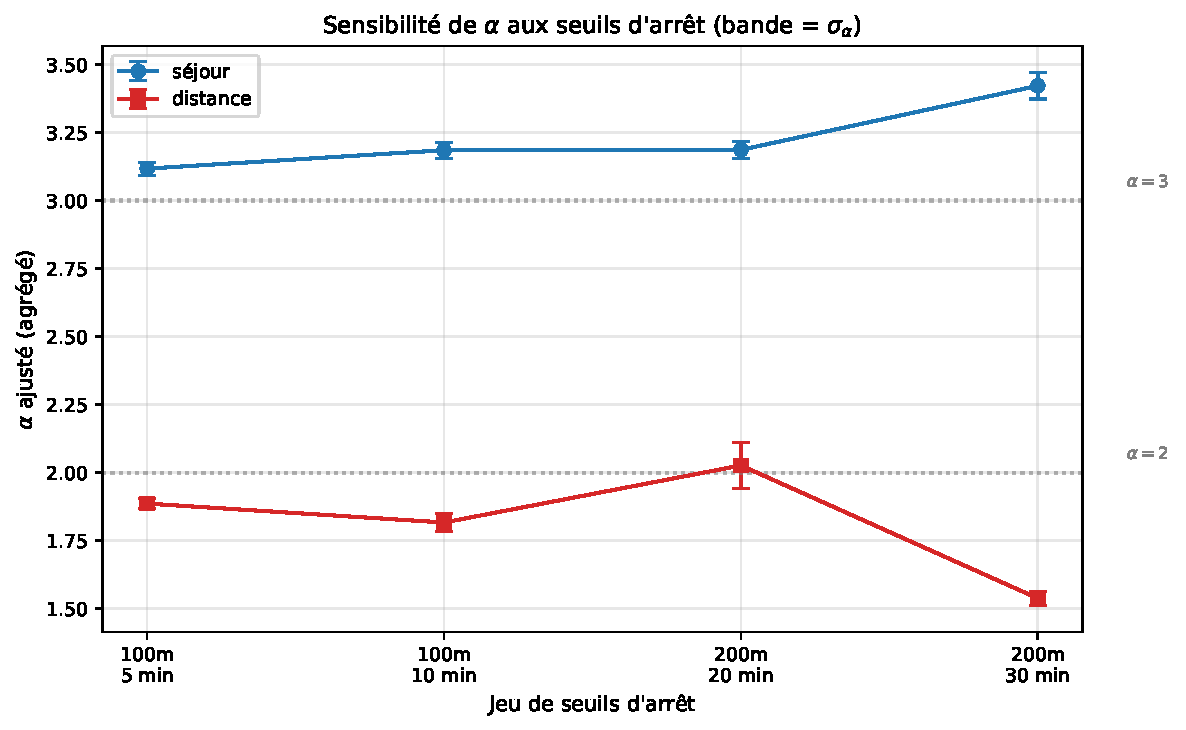
\includegraphics[width=0.85\linewidth]{graphe_12_sensibilite.pdf}
\caption{Sensibilité de l'exposant $\alpha$ aux quatre jeux de seuils d'arrêt
(population agrégée, barres d'erreur = $\sigma_\alpha$). La courbe « distance » porte sur
la distance à l'intérieur d'un même segment. L'exposant des séjours
reste au-dessus de 3 aux quatre jeux, donc hors du domaine $]2, 3[$ de la relation
ON/OFF. L'exposant des distances varie de 1{,}54 à 2{,}03 ; la
valeur basse du jeu 200~m~/~30~min repose sur $n = 428$ seulement.}
\label{fig:lp-sensibilite}
\end{figure}

L'exposant des séjours croît avec la durée minimale d'arrêt, de 3,12 à 3,42 : un seuil plus
exigeant élimine les séjours courts et durcit la queue. L'amplitude reste modérée
($\Delta\alpha = 0{,}30$), et surtout $\alpha_{\text{séjour}}$ reste au-dessus de 3 aux
quatre jeux, donc toujours hors du domaine $]2, 3[$ où la relation ON/OFF
$H = (4 - \alpha)/2$ s'applique. Ce résultat est robuste au choix de seuils. L'exposant des
distances est plus variable. La chute à 1,54 pour le jeu 200~m~/~30~min tient très
probablement à la taille de l'échantillon (428 paires seulement). Sur les trois jeux les
mieux fournis, $\alpha_{\text{distance}}$ reste dans $[1{,}82, 2{,}03]$. Toute valeur
d'$\alpha$ citée dans ce mémoire doit donc être accompagnée de son jeu de seuils. La
conclusion qualitative (la loi pure n'explique pas les séjours) ne change pas.

\subsubsection{Conséquence pour le lien ON/OFF}

La relation $H = (4-\alpha)/2$ ne vaut que pour $2 < \alpha < 3$, et elle ne s'applique
qu'à des \emph{durées} de phases ON/OFF. Nous ne pouvons donc la confronter qu'aux
variables de durée : \code{sejour} et \code{sejour\_avec\_censurees}. Le
tableau~\ref{tab:onoff-applique} résume l'examen.

\begin{table}[ht]
\centering
\caption{Application de la relation ON/OFF aux variables de durée. Les exposants de
distance ne sont pas des durées et ne relèvent pas de ce cadre.}
\label{tab:onoff-applique}
\small
\begin{tabular}{lrrll}
\toprule
Variable & $\alpha$ & Dans le domaine ? & $H_{\text{pred}}$ & Fiabilité \\
\midrule
\code{sejour} & $3{,}19$ & non ($\alpha > 3$) & --- & --- \\
\code{sejour\_avec\_censurees} & $2{,}37$ & \textbf{oui} & $0{,}817$ & très faible (bimodale probable) \\
\bottomrule
\end{tabular}
\end{table}

Aucun $H_{\text{pred}}$ calculable n'est solide. Pour \code{sejour\_avec\_censurees},
$H_{\text{pred}} \approx 0{,}82$ est du même ordre que les 0,726 mesurés par DFA, mais
la variable est probablement bimodale. L'écart apparent entre 0,82 et 0,726
\emph{pourrait} être cohérent avec la prédiction, mais l'hypothèse bimodale interdit de
le présenter comme une confirmation. Nous ne pouvons donc rien conclure, à ce stade, sur
la cohérence du lien ON/OFF avec les données réelles.

\subsubsection{Synthèse}

\begin{table}[ht]
\centering
\caption{Synthèse des résultats sur les lois de puissance.}
\label{tab:lp-synthese}
\small
\begin{tabular}{p{7.4cm}p{6.6cm}}
\toprule
Indicateur & Valeur \\
\midrule
Utilisateurs analysés (au moins un arrêt) & 137 \\
Jeu de seuils d'arrêt & 200~m~/~20~min \\
Loi pure mieux classée en AICc & \code{distance}, \code{sejour\_avec\_censurees} (poids 0,53 et 0,58) \\
Loi tronquée mieux classée en AICc & \code{sejour}, \code{distance\_a\_cheval} \\
Loi tronquée rejetée par le test d'adéquation & \code{sejour} \\
Cas ambigu & \code{distance} (même seg.) \\
Cas non interprétable (bimodale probable) & \code{sejour\_avec\_censurees} \\
$\alpha$ dans $]2,3[$ (domaine ON/OFF) & 2 variables sur 4 \\
$H_{\text{pred}}$ solide & aucun \\
\bottomrule
\end{tabular}
\end{table}

Le message à retenir est le suivant. La loi de puissance pure n'est pas confirmée sur ce
corpus. La loi tronquée est préférée en AICc sur deux variables, mais elle est rejetée par le
test d'adéquation sur la plus importante, \code{sejour}. L'échelle de coupure de 4,7~h
est proche du maximum observé et ne peut pas être interprétée de façon sûre. Le résultat est
donc double : un résultat négatif sur la modélisation (les deux lois soumises à un test
d'adéquation échouent, l'une au classement AICc, l'autre au bootstrap) et une piste, non un
acquis, vers une coupure exponentielle. Aucune prédiction ON/OFF solide ne peut être tirée.

% =====================================================================
\section{Discussion et perspectives}
\label{sec:discussion}
% =====================================================================

\subsection{Ce que le travail permet, et ce qu'il ne permet pas}

Le pipeline fournit, pour chaque segment, une estimation de $H$ accompagnée de drapeaux qui
disent dans quelle mesure elle est interprétable, et une précision de référence mesurée par
simulation. Il ne permet pas, à lui seul, de conclure à une mémoire longue : un dépassement
du modèle nul ne distingue pas mémoire longue et alternance de régimes, et un exposant
supérieur à 1 n'est pas une estimation de $H$.

\subsection{Limites d'ensemble}
\label{sec:limites}

\paragraph{Circularité et validité de construit.} Le filtre de fiabilité conditionne
l'estimation sur $H$ lui-même (section~\ref{sec:circularite}) : le $\hat H$ des segments
gardés est conditionnel, pas populationnel. De plus, la série des $d_i$ mélange vitesse et
intervalle de temps. Une valeur de $H$ est donc avant tout une propriété de la série et de
son prétraitement, pas nécessairement de la mobilité.

\paragraph{Mémoire longue, régimes et non-stationnarité.} Le test de dépassement ne distingue
pas mémoire longue et régimes~\cite{diebold2001}. Le test de stationnarité rejette presque
partout ($p<10^{-20}$ sur la quasi-totalité des segments gardés), et il peut le faire
même pour une série persistante stationnaire. Le $\hat H$ des gardés est donc un $H$
\emph{effectif}, pas celui d'un processus stationnaire.

\paragraph{Estimateurs.} La DFA est sensible aux tendances et aux ruptures~\cite{chen2002} ;
le R/S corrigé est biaisé à haute persistance, ce que nous avons mesuré ; le Whittle local
est limité à $H<1$ et se colle à une borne de la grille en cas de non-stationnarité.
Nous avons aussi souligné que le marquage des vitesses peut classer à tort en artefact un
trajet motorisé soutenu dans un segment surtout piéton (section~\ref{sec:prep}).

\paragraph{Un seul jeu de données exploitable.} T-Drive est incompatible avec l'estimation
de $H$ sur $d_i$ comme avec l'analyse des lois de puissance : ses arrêts correspondent au
stationnement nocturne des taxis, pas à des pauses fonctionnelles (section~\ref{sec:tdrive}).
Aucune analyse n'a donc pu être répliquée sur un second corpus.

\paragraph{Constantes.} Beaucoup de constantes sont des planchers ou des plafonds absolus
derrière des seuils relatifs (annexe~\ref{app:params}). Certaines sont définies mais non
utilisées par le code que nous avons examiné.

\paragraph{Lois de puissance.} Les résultats portent sur des données agrégées : une loi
tronquée agrégée n'implique pas que chaque individu suive une loi d'échelle~\cite{yan2013}.
Le test d'adéquation de la tronquée est moins exigeant que celui de Clauset, et seules deux
lois sur cinq ont un test d'adéquation. Le seuil de 300 points exclut 37 utilisateurs sans
justification pour cette analyse. Enfin, seuls 15 utilisateurs sur 137 ont au moins 100
séjours : c'est trop peu pour la typologie par ACP et K-means prévue au cahier des charges.
Trois options se présentent : abaisser le seuil à 50, utiliser \code{distance\_a\_cheval},
dont les observations sont plus nombreuses par utilisateur, ou renoncer à la typologie
quantitative. Cette décision reste à discuter avec l'encadrant.

\subsection{Perspectives}
\label{sec:perspectives}

\paragraph{Départager mémoire longue et régimes.} C'est la perspective la plus importante.
Le test de Berkes et al.~\cite{berkes2006}, dont l'hypothèse nulle est une mémoire courte avec
ruptures de moyenne, et celui de Qu~\cite{qu2011}, dont l'hypothèse nulle est une mémoire
longue stationnaire contre un régime ou une tendance, ont des hypothèses nulles opposées.
Leur combinaison (rejet du premier, non-rejet du second) fournirait une évidence convergente
en faveur de la DLP. On peut y ajouter l'invariance de $d$ par agrégation
temporelle~\cite{ohanissian2008}. Ces tests demandent d'abord que l'on mesure leur taille et
leur puissance par simulation sur des séries de longueur comparable aux nôtres, et de
préférence sur des segments longs. Un modèle nul à régimes, dérivé du nôtre, compléterait ce
dispositif.

\paragraph{Changer de série.} Nous proposons deux séries : une série à pas régulier,
obtenue en rééchantillonnant chaque segment, pour se placer en temps physique ; et une série
en temps d'événement, formée des distances entre arrêts successifs, qui se rapproche de celle
de Yan et al.~\cite{yan2014}. Pour cette dernière, la taille limite : avec environ 39
séjours par utilisateur en moyenne (5\,354 sur 137), il faudra regrouper les utilisateurs ou
se restreindre aux mieux fournis.

\paragraph{Mesurer le biais de sélection du filtre.} Passer des fGn de $H_0$ connu dans le
filtre de fiabilité et mesurer le biais qu'il induit est le test le plus critique pour
interpréter le 0,726. Il faudrait aussi estimer l'incertitude sur le $H$ global en
rééchantillonnant les utilisateurs plutôt que les segments, et quantifier la part de
segments gardés qui rejettent le modèle nul AR($p$), à $p_{\max}=1$ et $p_{\max}=5$.

\paragraph{Contrôler l'effet de mélange sur les lois.} On peut simuler, pour chaque
utilisateur, des durées exponentielles de même effectif et de même moyenne, relancer
exactement la chaîne d'analyse, et comparer $\alpha$, la $p$-valeur et le meilleur modèle à
ceux observés. Si les valeurs observées sortent de la dispersion du modèle simulé, on
disposerait d'un indice de queues lourdes individuelles ; sinon, les résultats seraient
indiscernables d'un simple mélange. On pourrait aussi tester l'adéquation des trois autres
lois, harmoniser la procédure des deux tests d'adéquation, et vérifier la bimodalité de
\code{sejour\_avec\_censurees} par un histogramme log-log des durées. Enfin, relancer l'analyse
avec un seuil de 50 points quantifierait le biais d'exclusion des 37 utilisateurs.

\paragraph{Exploiter les labels de transport.} Un segment qui mélange plusieurs modes est un
changement de régime de vitesse, donc une source de confusion avec la mémoire longue. Les
labels (69 utilisateurs) permettraient de couper aux changements de classe (marche, vélo,
véhicule routier, bus, rail, avion, bateau), d'estimer $\hat H$ par mode, de disposer d'une
vérité terrain partielle pour le détecteur d'artefacts, et de remplacer le seuil unique de
200~km/h par des quantiles par classe. Les limites attendues sont la couverture partielle,
la qualité incertaine de labels saisis à la main, la fragmentation des segments et une
circularité possible si les mêmes labels servent à couper et à évaluer.

\paragraph{Améliorations méthodologiques.} Corriger la simulation ON/OFF, puis relancer la
comparaison sur données réelles. Passer au Whittle local exact de Shimotsu et Phillips, avec
une bande passante variable. Séparer le traitement en deux branches (segments continus pour
$H$, chronologie par utilisateur pour les séjours), fusionner les arrêts proches et écrire
la vraisemblance avec censure. Réaliser enfin la typologie des utilisateurs et la
cartographie des zones de mémoire, puis étendre l'analyse à d'autres jeux de données.

% =====================================================================
\section{Conclusion}
\label{sec:conclusion}
% =====================================================================

Ce mémoire présente une chaîne complète, du fichier GPS brut à l'ajustement de lois de
puissance, avec un principe : ne jamais cacher ce qui limite l'interprétation. Les points
suspects sont marqués plutôt que supprimés, les durées censurées sont étiquetées, les
estimations hors domaine sont signalées, le test de dépassement est accompagné de la mesure
de ses faux positifs, et la circularité du filtre de fiabilité est explicitée.

Sur l'exposant de Hurst, nos résultats (19\,150 segments retenus, 7\,853 gardés,
$\hat H_{\mathrm{DFA}}\approx 0{,}726$ sur les gardés) ne démontrent pas la mémoire longue du
déplacement humain. Ils quantifient une persistance locale dont la robustesse aux régimes et
au bruit d'échantillonnage n'est pas établie. La question reste ouverte. Pour la trancher,
il faudra une série d'un autre type (événements, agrégats spatio-temporels) et des tests qui
distinguent mémoire longue et régimes. Ce que nous pouvons affirmer est modeste : sur des
segments filtrés de GeoLife, la DFA appliquée à la série des distances inter-points donne
environ $0{,}726$ ; ce chiffre ne mesure pas la dépendance à longue portée du déplacement.

Sur les lois de puissance, l'analyse de 137 utilisateurs donne un résultat négatif partiel
mais solide. La loi de puissance pure n'est pas confirmée : elle est rejetée pour trois
variables sur quatre. La loi à coupure exponentielle est préférée en AICc pour les durées de
séjour et pour les distances à cheval (poids de 0,97 et 0,51), mais un test d'adéquation la
rejette pour les séjours ($p<0{,}005$) ; son $p=1{,}000$ pour les distances à cheval est un
artefact d'un $\lambda$ numériquement nul. L'échelle de coupure des séjours, environ 4,7~h,
est proche de la durée maximale observée et ne peut pas être interprétée avec certitude.
Ni la loi pure (non rejetée par Clauset mais battue en AICc) ni la loi tronquée (préférée en
AICc mais rejetée par bootstrap) ne décrit correctement les durées de séjour. Le cas des
distances dans un même segment reste ambigu ($p=0{,}055$) et les séjours avec censurés sont
probablement bimodaux. Enfin, la relation ON/OFF $H=(4-\alpha)/2$ ne peut être testée de
façon fiable sur aucune variable de durée : les deux exposants situés dans le domaine
$]2,3[$ reposent l'un sur un modèle rejeté, l'autre sur une distribution probablement
bimodale.

% =====================================================================
\appendix
\section{Paramètres du pipeline}
\label{app:params}
% =====================================================================

Les valeurs listées correspondent au fichier de configuration au moment de la rédaction
(\code{TIME\_GAP\_THRESHOLD = 900}). La colonne « Statut » distingue : \textbf{conv.}
(convention de la littérature), \textbf{emp.} (valeur empirique à calibrer), \textbf{dév.}
(interrupteur de développement) et \textbf{num.} (paramètre numérique). Le symbole $\dagger$
signale une constante définie dans la configuration mais non utilisée par le code que nous
avons examiné.

{\small
\begin{longtable}{@{}p{4.9cm}p{1.9cm}p{6.2cm}p{1.1cm}@{}}
\caption{Constantes de la configuration.}\label{tab:params}\\
\toprule
Constante & Valeur & Rôle & Statut \\
\midrule
\endfirsthead
\toprule
Constante & Valeur & Rôle & Statut \\
\midrule
\endhead
\bottomrule
\endfoot
\multicolumn{4}{@{}l}{\textit{Segmentation et sélection}}\\
\code{TIME\_GAP\_THRESHOLD} & 900 s & trou qui coupe un segment & emp.\\
\code{MIN\_POINTS} & 300 & points minimaux d'un segment retenu & emp.\\
\code{MIN\_POINTS\_MORCEAU} & 50 & points minimaux d'un morceau & emp.\\
\code{DISTANCE\_MIN} & 0{,}1 km & distance minimale d'un segment retenu & emp.\\
\code{DISTANCE\_MIN\_RELATIF} & True & seuil relatif au pas d'échantillonnage & emp.\\
\multicolumn{4}{@{}l}{\textit{Marquage}}\\
\code{MAX\_SPEED} & 200 km/h & plafond absolu du seuil de vitesse (seuil effectif : $\min(200,\max(5,20\tilde v))$) & emp.\\
\code{MAX\_SPEED\_RELATIF} & 20 & multiple de la vitesse médiane & emp.\\
\code{MAX\_DIST\_M} & 30 & multiple de la distance médiane (mode relatif) & emp.\\
\code{MAX\_DIST\_M\_ABSOLU} & 500 m & plafond absolu du seuil de distance & emp.\\
\code{MODE\_MAX\_DIST} & relatif & mode du filtre de distance & dév.\\
\code{ORDRE\_FILTRES} & distance\_puis\_vitesse & ordre d'application & dév.\\
\code{MAD\_Z\_SEUIL} & 3,5 & seuil du Z-score modifié & conv.\\
\code{MAD\_PERSISTANCE\_MIN} & 5 & plancher de persistance & emp.\\
\code{MAD\_PERSISTANCE\_FRACTION} & 0{,}01 & fraction de la longueur & emp.\\
\code{MAD\_DELTA\_V\_BRUTAL} & 20 km/h & plancher de variation brutale & emp.\\
\code{MAD\_DELTA\_V\_FACTEUR\_MAD} & 5 & multiple de $\mathrm{MAD}_v$ & emp.\\
\code{MAD\_R\_HETEROGENE} & 1{,}5 & seuil du ratio $R$ & emp.\\
\code{MAD\_R\_TEST\_NUL} & True & test contre la loi nulle & emp.\\
\code{MAD\_FALLBACK\_SPEED} & 5 km/h & plancher si MAD nul & emp.\\
\code{MAD\_FALLBACK\_SPEED\_FACTEUR} & 3 & multiple de la vitesse médiane & emp.\\
\multicolumn{4}{@{}l}{\textit{Stationnarité}}\\
\code{STATIO\_TEST} & ks & test KS (remplace le ratio) & emp.\\
\code{STATIO\_ALPHA} & 0{,}05 & seuil du test & conv.\\
\code{STATIO\_MIN\_POINTS} & 10 & points minimaux par moitié & emp.\\
\code{STATIO\_RATIO\_MIN}, \code{STATIO\_RATIO\_MAX} & 0{,}7 ; 1{,}4 & affichage seulement & emp.\\
\multicolumn{4}{@{}l}{\textit{Estimateurs de $H$}}\\
\code{SERIE\_ANALYSEE} & distance & série analysée & dév.\\
\code{N\_S} & 20 & nombre d'échelles DFA & conv.\\
\code{DFA\_ECHELLE\_MIN} & 4 & plus petite échelle DFA & emp.\\
\code{DFA\_DIVISEUR\_ECHELLE\_MAX} & 4 & $s_{\max}=N/4$ & conv.\\
\code{DFA\_ORDRE} & 1 & ordre du détrendage & conv.\\
\code{DFA\_FENETRE\_PENTES\_LOCALES} & 5 & échelles par pente locale & dév.\\
\code{DFA\_N\_MIN}$^\dagger$ & 16 & points minimaux DFA & emp.\\
\code{N\_M} & 20 & nombre de tailles de bloc R/S & conv.\\
\code{M\_MIN\_RS} & 10 & plus petite taille de bloc R/S & conv.\\
\code{M\_MIN\_RS\_DIVISEUR}$^\dagger$ & 20 & prévu pour $m_{\min}=\max(10, N/20)$ & emp.\\
\code{RS\_DIVISEUR\_M\_MAX} & 2 & $m_{\max}=N/2$ & conv.\\
\code{K\_WHITTLE} & 1000 & taille de la grille de $H$ & num.\\
\code{N\_MIN\_WHITTLE} & 20 & plancher technique pour le Whittle & conv.\\
\code{N\_MIN\_WHITTLE\_M\_CIBLE}$^\dagger$ & 8 & $m$ minimal cible & emp.\\
\code{WHITTLE\_EXPOSANT\_M} & 0{,}65 & $m=N^{0{,}65}$ & emp.\\
\code{WHITTLE\_DIVISEUR\_M\_MAX} & 4 & $m\le N/4$ & conv.\\
\multicolumn{4}{@{}l}{\textit{Test de dépassement}}\\
\code{AVEC\_TEST\_NUL} & True & test calculé pour chaque segment & dév.\\
\code{NUL\_MODELE} & ar & modèle nul & dév.\\
\code{NUL\_NB\_SURROGATS} & 99 & surrogats par segment & conv.\\
\code{NUL\_ORDRE\_AR\_MAX} & 5 & ordre maximal $p$ & emp.\\
\code{NUL\_ALPHA} & 0{,}05 & seuil du test & conv.\\
\code{GRAINE} & 20261018 & graine de toute simulation & dév.\\
\multicolumn{4}{@{}l}{\textit{Mode d'enregistrement}}\\
\code{ECHANT\_TOL\_DT} & 0{,}2 & tolérance sur le pas de temps & emp.\\
\code{ECHANT\_TOL\_D} & 0{,}3 & tolérance sur la distance & emp.\\
\code{ECHANT\_PART\_TEMPS} & 0{,}6 & part minimale du mode temps & emp.\\
\code{ECHANT\_PART\_DISTANCE} & 0{,}5 & part minimale du mode distance & emp.\\
\code{ECHANT\_DEPLACEMENT\_MIN\_M} & 1 m & seuil « en mouvement » & emp.\\
\code{ECHANT\_MIN\_MOUVEMENT}$^\dagger$ & 10 & points minimaux en mouvement & emp.\\
\multicolumn{4}{@{}l}{\textit{Arrêts}}\\
\code{ARRET\_RAYON\_M} & 200 m & rayon d'arrêt & emp.\\
\code{ARRET\_DUREE\_MIN\_S} & 1200 s & durée minimale d'un arrêt & emp.\\
\code{ARRET\_TROU\_MAX\_S} & 900 s & trou qui coupe la série & emp.\\
\code{ARRET\_RAYON\_PAUSE\_M} & 200 m & rayon d'une pause entre segments & emp.\\
\code{ARRET\_DISTANCE\_MIN\_M} & 100 m & distance minimale entre deux arrêts & emp.\\
\code{ARRET\_JEUX\_SENSIBILITE} & (100,300) à (200,1800) & 4 couples testés & dév.\\
\multicolumn{4}{@{}l}{\textit{Lois de puissance}}\\
\code{LP\_NB\_CANDIDATS\_XMIN} & 200 & seuils $x_{\min}$ essayés & num.\\
\code{LP\_NB\_MIN\_QUEUE} & 50 & taille minimale de la queue & emp.\\
\code{LP\_NB\_BOOTSTRAP} & 1000 & simulations de bootstrap (test de Clauset) & emp.\\
\code{LP\_SEUIL\_P} & 0{,}1 & seuil de rejet~\cite{clauset2009} & conv.\\
\code{LP\_NB\_MIN\_PAR\_UTILISATEUR} & 100 & observations minimales par utilisateur & emp.\\
\end{longtable}
}

% =====================================================================
\section{Abréviations et notations}
\label{app:abrev}
% =====================================================================

\begin{table}[H]
\centering
\caption{Abréviations et notations.}
\small
\begin{tabular}{@{}p{3.2cm}p{11.3cm}@{}}
\toprule
Sigle & Signification \\
\midrule
AIC, AICc & critère d'information d'Akaike, et sa version corrigée pour les petits échantillons \\
AR($p$) & modèle autorégressif d'ordre $p$ \\
ACP & analyse en composantes principales \\
DFA & analyse des fluctuations redressées (\emph{detrended fluctuation analysis}) \\
DLP (LRD) & dépendance à longue portée (\emph{long-range dependence}) \\
fBm, fGn & mouvement brownien fractionnaire, bruit gaussien fractionnaire \\
GPS & système de positionnement par satellite \\
$H$ & exposant de Hurst \\
i.i.d. & indépendantes et identiquement distribuées \\
KS & Kolmogorov--Smirnov \\
LP (dans les figures) & loi de puissance \\
MAD & déviation absolue médiane \\
ON/OFF & alternance de phases de mouvement (ON) et d'arrêt (OFF) \\
R/S & analyse de l'étendue normalisée (\emph{rescaled range}) \\
RMSE & racine de l'erreur quadratique moyenne \\
$\rho_1$, $\rho_S$ & autocorrélation de retard 1 ; corrélation de Spearman \\
$x_{\min}$, $\alpha$, $\lambda$ & seuil de la queue, exposant de densité, taux de coupure exponentielle \\
\bottomrule
\end{tabular}
\end{table}

% =====================================================================
\section{Scripts et organisation du code}
\label{app:scripts}
% =====================================================================

\begin{itemize}
  \item \code{00\_audit\_echantillonnage.py} : audit des intervalles d'échantillonnage.
  \item \code{01\_pretraitement.py} : chaîne de prétraitement, un fichier CSV par utilisateur.
  \item \code{02\_validation\_methodes.py} : validation sur séries synthétiques.
  \item \code{03\_estimation\_H.py} : estimation de $H$ par segment et drapeaux de fiabilité.
  \item \code{H\_valides.py} : filtre de fiabilité (fichiers \code{<user>\_H\_gardes.csv} et
  \code{synthese\_H.csv}).
  \item \code{04\_lois\_de\_puissance.py} : point d'entrée des lois de puissance (mode démo
  synthétique, mode analyse rapide, mode complet) ; délègue à
  \code{experiences/lois\_de\_puissance.py} la détection d'arrêts et l'analyse agrégée.
  \item \code{audit\_grille.py}, \code{audit\_time\_gap.py}, \code{audit\_users.py},
  \code{audit\_survivants.py} : audits de calibration et de sélection.
  \item \code{experiences/} : sensibilité, lois de puissance, mécanisme ON/OFF, validation
  visuelle, analyse de T-Drive.
  \item \code{graphes.py} : génération des figures (sorties PDF dans \code{figures/}).
  \item \code{simulation/}, \code{validation/}, \code{hurst/}, \code{lois\_de\_puissance/},
  \code{pretraitement/} : modules ; \code{tests/} : tests automatiques (parité, estimateurs,
  arrêts, lois de puissance).
\end{itemize}

% =====================================================================
\begin{thebibliography}{99}
\addcontentsline{toc}{section}{Références}
% =====================================================================

\bibitem{peng1994} C.-K. Peng et al. Mosaic organization of DNA nucleotides. \textit{Physical Review E}, 49(2):1685--1689, 1994.
\bibitem{hurst1951} H.~E. Hurst. Long-term storage capacity of reservoirs. \textit{Transactions of the American Society of Civil Engineers}, 116:770--799, 1951.
\bibitem{mandelbrot1968} B.~B. Mandelbrot, J.~W. Van Ness. Fractional Brownian motions, fractional noises and applications. \textit{SIAM Review}, 10(4):422--437, 1968.
\bibitem{mandelbrot1969} B.~B. Mandelbrot, J.~R. Wallis. Robustness of the rescaled range R/S. \textit{Water Resources Research}, 5(5):967--988, 1969.
\bibitem{anis1976} A.~A. Anis, E.~H. Lloyd. The expected value of the adjusted rescaled Hurst range. \textit{Biometrika}, 63(1):111--116, 1976.
\bibitem{lo1991} A.~W. Lo. Long-term memory in stock market prices. \textit{Econometrica}, 59(5):1279--1313, 1991.
\bibitem{weron2002} R. Weron. Estimating long-range dependence. \textit{Physica A}, 312:285--299, 2002.
\bibitem{robinson1995} P.~M. Robinson. Gaussian semiparametric estimation of long range dependence. \textit{The Annals of Statistics}, 23(5):1630--1661, 1995.
\bibitem{phillips2004} P.~C.~B. Phillips, K. Shimotsu. Local Whittle estimation in nonstationary and unit root cases. \textit{The Annals of Statistics}, 32(2), 2004.
\bibitem{shimotsu2005} K. Shimotsu, P.~C.~B. Phillips. Exact local Whittle estimation of fractional integration. \textit{The Annals of Statistics}, 33(4), 2005.
\bibitem{davies1987} R.~B. Davies, D.~S. Harte. Tests for Hurst effect. \textit{Biometrika}, 74(1):95--101, 1987.
\bibitem{maraun2004} D. Maraun, H.~W. Rust, J. Timmer. Tempting long-memory. \textit{Nonlinear Processes in Geophysics}, 11(4):495--503, 2004.
\bibitem{chen2002} Z. Chen et al. Effect of nonstationarities on detrended fluctuation analysis. \textit{Physical Review E}, 65:041107, 2002.
\bibitem{katsev2003} S. Katsev, I. L'Heureux. Are Hurst exponents estimated from short or irregular time series meaningful? \textit{Computers \& Geosciences}, 29(9):1085--1089, 2003.
\bibitem{diebold2001} F.~X. Diebold, A. Inoue. Long memory and regime switching. \textit{Journal of Econometrics}, 105(1):131--159, 2001.
\bibitem{berkes2006} I. Berkes, L. Horváth, P. Kokoszka, Q.-M. Shao. On discriminating between long-range dependence and changes in mean. \textit{The Annals of Statistics}, 34(3):1140--1165, 2006.
\bibitem{qu2011} Z. Qu. A test against spurious long memory. \textit{Journal of Business \& Economic Statistics}, 29(3):423--438, 2011.
\bibitem{ohanissian2008} A. Ohanissian, J.~R. Russell, R.~S. Tsay. True or spurious long memory? A new test. \textit{Journal of Business \& Economic Statistics}, 26(2):161--175, 2008.
\bibitem{clauset2009} A. Clauset, C.~R. Shalizi, M.~E.~J. Newman. Power-law distributions in empirical data. \textit{SIAM Review}, 51(4):661--703, 2009.
\bibitem{vuong1989} Q.~H. Vuong. Likelihood ratio tests for model selection and non-nested hypotheses. \textit{Econometrica}, 57(2):307--333, 1989.
\bibitem{burnham2002} K.~P. Burnham, D.~R. Anderson. \textit{Model Selection and Multimodel Inference}. Springer, 2002.
\bibitem{kivela2015} M. Kivelä, M.~A. Porter. Estimating interevent time distributions from finite observation periods in communication networks. \textit{Physical Review E}, 92:052813, 2015.
\bibitem{taqqu1997} M.~S. Taqqu, W. Willinger, R. Sherman. Proof of a fundamental result in self-similar traffic modeling. \textit{ACM SIGCOMM Computer Communication Review}, 27(2):5--23, 1997.
\bibitem{brockmann2006} D. Brockmann, L. Hufnagel, T. Geisel. The scaling laws of human travel. \textit{Nature}, 439:462--465, 2006.
\bibitem{gonzalez2008} M.~C. González, C.~A. Hidalgo, A.-L. Barabási. Understanding individual human mobility patterns. \textit{Nature}, 453:779--782, 2008.
\bibitem{song2010} C. Song, T. Koren, P. Wang, A.-L. Barabási. Modelling the scaling properties of human mobility. \textit{Nature Physics}, 6:818--823, 2010.
\bibitem{yan2013} X.-Y. Yan, X.-P. Han, B.-H. Wang, T. Zhou. Diversity of individual mobility patterns and emergence of aggregated scaling laws. \textit{Scientific Reports}, 3:2678, 2013.
\bibitem{rhee2011} I. Rhee et al. On the Lévy-walk nature of human mobility. \textit{IEEE/ACM Transactions on Networking}, 19(3):630--643, 2011.
\bibitem{yan2014} X.-Y. Yan, X.-P. Han, B.-H. Wang, T. Zhou. Correlations and scaling laws in human mobility. \textit{PLoS ONE}, 9(1):e84954, 2014.
\bibitem{eke2002} A. Eke, P. Herman, L. Kocsis, L.~R. Kozak. Fractal characterization of complexity in temporal physiological signals. \textit{Physiological Measurement}, 23(1):R1--R38, 2002.
\bibitem{iglewicz1993} B. Iglewicz, D.~C. Hoaglin. \textit{How to Detect and Handle Outliers}. ASQC Quality Press, 1993.
\bibitem{li2008} Q. Li et al. Mining user similarity based on location history. In \textit{Proc. ACM SIGSPATIAL GIS}, 2008.
\bibitem{zheng2009} Y. Zheng et al. Mining interesting locations and travel sequences from GPS trajectories. In \textit{Proc. WWW}, 2009, p.~791--800.
\bibitem{zheng2010} Y. Zheng, X. Xie, W.-Y. Ma. GeoLife: a collaborative social networking service. \textit{IEEE Data Engineering Bulletin}, 33(2):32--40, 2010.
\bibitem{geolifeguide} Microsoft Research Asia. \textit{GeoLife GPS Trajectories --- User Guide}, version 1.2, 31 octobre 2011.

\end{thebibliography}

\end{document}